\chapter{Σχεδίαση Συστήματος}
\label{chap4}

Στο προηγούμενο κεφάλαιο έγινε μια εισαγωγική αναφορά στα δομικά μέρη του συστήματος της εφαρμογής, δηλάδή του \tl{frontend} (\tl{client}) και του \tl{backend} (\tl{server} και βάση δεδομένων). Αναπτύχθηκαν οι λειτουργικότητες της εφαρμογής και οι αντίστοιχες οθόνες που θα τις καλύπτουν. Επίσης, έγινε μια αναφορά στα συστατικά του \tl{server} και πως αυτά αλληλεπιδρούν με τη βάση δεδομένων για την λήψη και αποστολή δεδομένων από και προς τον \tl{client}.

Αυτό το κεφάλαιο θα επικεντρωθεί στην σχεδίαση των υποδομών της εφαρμογής. Συγκεκριμένα, θα γίνει αναφορά στις διεπιφάνειες που θα συνιστούν κάθε οθόνη της εφαρμογής και θα παρουσιαστούν τα διαγράμματα ροής για τα σενάρια χρήσης της εφαρμογής (βλ. ενότητα 4.1). Στην ενότητα 4.2, θα γίνει αναφορά στην πλευρά του \tl{server}. Θα παρουσιαστεί η διαδικασία σχεδίασης των εξυπηρετητών αιτημάτων και θα μελετηθούν οι τακτικές και οι τεχνολογίες που χρησιμοποιήθηκαν. Τέλος, στην ενότητα 4.3, θα γίνει μια εκτενής ανάλυση του τρόπου με τον οποίο σχεδιάστηκε η βάση δεδομένων για να ανταποκρίνεται βέλτιστα στις απαιτήσεις της εφαρμογής.

\section{Σχεδίαση Μοντέλων των Διεπιφανειών της Εφαρμογής}
Όπως έχει ήδη αναφερθεί, η εφαρμογή αποτελείται από οθόνες, καθεμία εκ των οποίων συνιστά και μια διεπαφή χρήστη. Σε αυτή την ενότητα θα αναλυθούν οι τεχνικές σχεδίασης των διεπαφών χρήστη και θα παρουσιαστούν παραστατικά διαγράμματα των συστατικών μερών τους.

\subsection{Αρχιτεκτονική Σχεδίασης Οθονών}
Κατα την σχεδίαση μιας \tl{mobile} εφαρμογής, ο προγραμματιστής καλείται να αποφανθεί σχετικά με τον τρόπο διαμερισμού του εσωτερικού της εφαρμογής (\tl{compartmentalization}). Τα δομικά μέρη της εφαρμογής θεωρούνται ως εξαρτήματα, τα οποία στο σύνολό τους συνθέτουν μεγαλύτερα τμήματα της εφαρμογής. Τέτοια εξαρτήματα είναι τα πλήκτρα ενεργειών, τα μενού, οι διεπαφές εισόδου και όλα τα διαδραστικά στοιχεία της εφαρμογής. Η κατάλληλη διασύνδεση μεταξύ πολλών διαδραστικών στοιχείων διαμορφώνει μια διεπιφάνεια χρήστη. Η διεπιφάνειες χρήστη ή αλλιώς κλάσεις, αποτελούν το κύριο συνθετικό στοιχείο (\tl{component}) μιας οθόνης της εφαρμογής. Κάθε οθόνη περιλαμβάνει διαφορετικές κλάσεις, οι οποίες εξυπηρετούν διαφορετικούς σκοπούς. Για παράδειγμα, η οθόνη εγγραφής/σύνδεσης του χρήστη στην εφαρμογή αποτελείται από μια διεπαφή ατυτοποίησης, η οποία περιέχει μια φόρμα με πολλαπλά στοιχεία εισόδου κειμένου, πλήκτρα και μηνύματα. η κεντρική οθόνη της εφαρμογής συνίσταται από μια διεπαφή χάρτη, η οποία αποτελεί τη διεπιφάνεια προβολής όλων των \tl{hotspots} και περιέχει \tl{markers} για καθένα από τα \tl{hotspots}.\newline
\indent
Είναι προφανές λοιπόν πως, αν και η οθόνη ταυτοποίησης χρήστη διαφέρει ως προς το σκοπό της από την οθόνη χάρτη, η δομή τους ακολουθεί μια ομοιόμορφη αρχιτεκτονική σχεδίασης. Στη συνέχεια, θα γίνει μια αναλυτική αναφορά στις μεθόδους που χρησιμοποιήθηκαν κατά τη σχεδίαση των οθονών της εφαρμογής και θα παρουσιαστούν τα μοντέλα κάθε διεπιφάνειας.

\subsection{Λογική Σχεδίασης και Ροή Πληροφορίας Μεταξύ οθονών}
Η λογική σχεδίασης που ακολουθεί η εφαρμογή διακρίνεται σε 5 στάδια, τα οποια σειριοποιούνται ως εξής:
\begin{enumerate}
    \item οθόνη έναρξης
    \item ταυτοποίηση χρήστη
    \item κεντρική οθόνη
    \item οθόνες μηνυμάτων και αλληλεπίδρασης
    \item προσωπικός λογαριασμός και ρυθμίσεις 
\end{enumerate}

Το μοντέλο αυτό ροής της πληροφορίας (βλ. Σχ. \ref{pageflow}) ακολουθείται από την πλειοψηφία των σημερινών εφαρμογών. Κατά τη διαδικασία εξερεύνησης της εφαρμογής, ο χρήστης εισάγεται στον τρόπο λειτουργίας της εφαρμογής σταδιακά. Κάθε στάδιο προσφέρει στο χρήστη εμπειρία συγκεκριμένου τύπου, χωρίς να τον επιβαρρύνει με αχρείαστες υπηρεσίες. Ο χρήστης θα πρέπει να μπορεί να αποκτήσει εμπειρία άμεσα. Η εκμάθηση της εφαρμογής θα πρέπει να είναι εύκολη και αβίαστη και όχι να δημιουργεί την αίσθηση ανικανότητας ή δυσκολίας χειρισμού. \newline
\indent
Επίσης, κάθε σημείο της εφαρμογής θα πρέπει να είναι εύκολα προσβάσιμο από κάθε οθόνη της εφαρομογής. Για το λόγο αυτό κάθε οθόνη πρέπει να περιλαμβάνει μια επικεφαλίδα με πλήκτρα πλοήγησης και χαρακτηριστικά γνωρίσματα που ενημερώνουν το χρήστη για το την πορεία του εντός της εφαρμογής.


\begin{figure}[H]
    \centering
    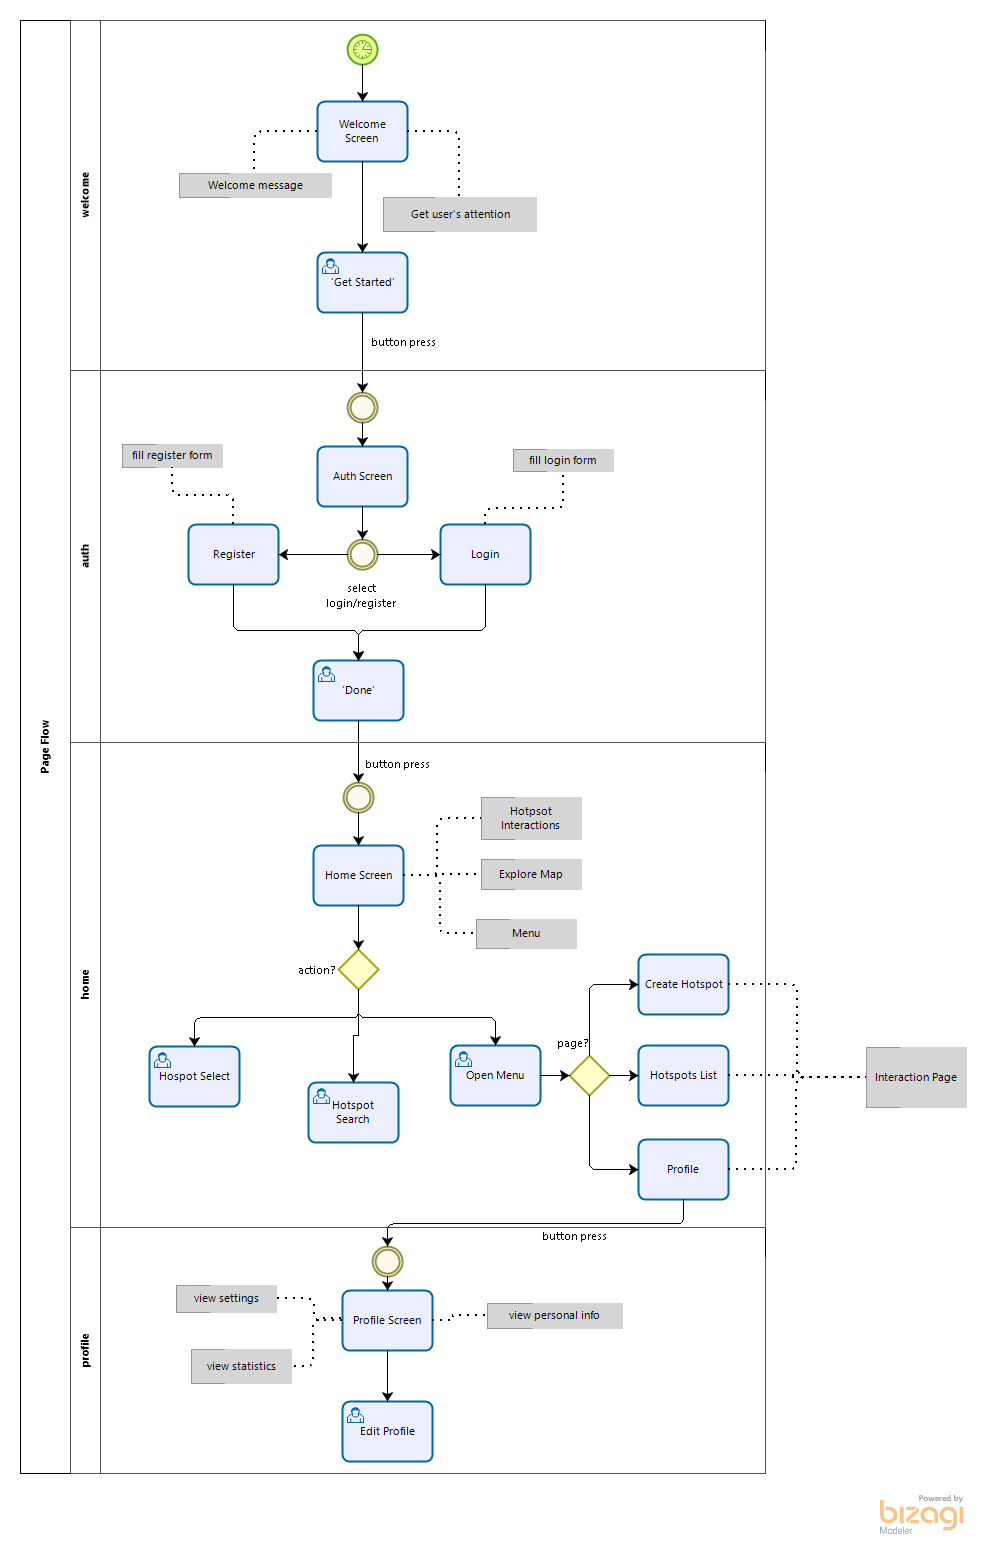
\includegraphics[scale=0.6]{figures/page-flow.png}
    \caption{Ροή πληροφορίας μεταξύ οθονών της εφαρμογής.}
    \label{pageflow}
\end{figure}


Στο πρώτο στάδιο της εφαρμογής, ο χρήστης εισάγεται με άμεσο και σύντομο τρόπο στο νόημα της εφαρμογής. Ένα φιλικό μήνυμα καλωσορίσματος εξυπηρετεί στη διαμόρφωση μιας θετικής πρώτης εντύπωσης στο χρήστη. Το μόνο απαραίτητο διαδραστικό μέσο είναι το πλήκτρο που θα μεταφέρει το χρήστη στο επόμενο στάδιο. \newline
\indent
Το στάδιο ταυτοποίησης του χρήστη απαρτίζεται από δύο σελίδες. Η πρώτη σελίδα αποτελείται από τη φόρμα εγγραφής, ενώ η δεύτερη διαθέτει μια φόρμα σύνδεσης. Και οι δύο σελίδες συνοδεύονται από ένα πλήκρο υποβολής. Κάθε φόρμα θα πρέπει να είναι σαφής, τόσο ως προς τα στοιχεία που απαιτεί από το χρήστη, όσο και ως προς τον τρόπο συμπλήρωσής της. Για το λόγο αυτό γίνεται χρήση διευκρυνιστικών τίτλων, παραδειγμάτων εισόδου και άλλων μηνυμάτων τέτοιου σκοπού. Επίσης, θα πρέπει να ληφθούν υπόψη πιθανά σφάλματα που μπορεί προκύψουν, όπως η αγνόηση ενός ή περισσότερων σημείων εισόδου, η λανθασμένη συμπλήρωση ενός ή περισσότερων κελιών, ο λανθασμένος συνδυασμός διαπιστευτηρίων του χρήστη κλπ. Η εφαρμογή θα διαθέτει μια πλήρως καταρτισμένη και εξυπηρετική διεπαφή εμφάνισης μηνυμάτων λάθους στο χρήστη, με σκοπό την εύκολη διόρθωση σφαλμάτων και τη γρήγορη σύνδεση/εγγραφή στην εφαρμογή. \newline
\indent
Η κεντρική οθόνη είναι το πιο σύνθετο στάδιο της εφαρμογής. Αποτελείται από πολλά διαδραστικά στοιχεία και διεπαφές χρήστη, οι κυριότερες εκ των οποίων είναι ο χάρτης των \tl{hotspots}, η μπάρα αναζήτησης, το μενού πλοήγησης και το μενού επιλογής φίλτρων. Αν και η πολυπλοκότητα είναι υψηλή, οι αντίστοιχες διεπιφάνειες είναι σχεδιασμένες με τέτοιο τρόπο, ώστε να απλοποιούν τις ενέργειες που απαιτούνται από το χρήστη. Εικονίδια, τίτλοι και βοηθητικές περιγραφές χρησιμοποιούνται καθ' όλη την έκταση της κεντρικής σελίδας. Τα μηνύματα είναι σύντομα, χρησιμοποιώνντας όσο το δυνατόν λιγότερους χαρακτήρες για να διευκολύνουν το χρήστη και να δημιουργούν μια εύχρηστη και ευανάγνωστη διεπιφάνεια. Άλλωστε, ο χώρος στην οθόνη μιας κινητής συσκευής είναι εξαρχής περιορισμένος και δεν ευνοεί το συνωστισμό πληροφοριών σε ένα σημείο ή την υπερβολική λεπτομέρεια στο σχεδιασμό.\newline
\indent
Το ενδιάμεσο στάδιο ορίζεται από τις οθόνες αλληλεπίδρασης του χρήστη με τις εξειδικευμένες υπηρεσίες που προσφέρει η εφαρμογή. Η οθόνη γρήγορης προβολής ενός \tl{hotspot}, η οθόνη προβολής λεπτομερειών ενός \tl{hotspot}, η οθόνη δημιουργίας ενός \tl{hotspot} και η οθόνη λίστας προσωπικών \tl{hotspots} του χρήστη αποτελούν το πεδίο δράσης του χρήστη. Οι οθόνες αυτές διαμορφώνουν τη φυσιογνωμία της εφαρμογής και τη διακρίνουν από τις υπόλοιπες εφαρμογές, με τις μοναδικές λειτουργικότητες που προσφέρουν. \newline
\indent
Τέλος, το στάδιο του προσωπικού λογαριασμού αποτελείται από τις οθόνες που αφορούν τα προσωπικά στοιχεία του χρήστη. Οι οθόνες αυτές είναι σχεδιασμένες έτσι ώστε να προσφέρουν με άμεσο και σύντομο αλλά περιεκτικό τρόπο μια εικόνα του λογαριασμού του εκάστοτε χρήστη. Επιπλέον, ο χρήστης έχει τη δυνατότητα να προβάλλει επιπρόσθετα στοιχεία που αφορούν τη δράση του εντός της εφαρμογής. Στην οθόνη του προσωπικού λοαγιασμού, ο χρήστης μπορεί να τροποποιήσει τις προσωπικές του ρυθμίσεις, καθώς και να επεξεργαστεί τα προσωπικά του στοιχεία.

\subsection{Διεπαφές Μηνυμάτων Προς το Χρήστη}
Η εφαρμογή είναι σχεδιασμένη ώστε να επιτρέπει τη μέγιστη δυνατή ευελιξία στο χρήστη εντός της εφαρμογής. Ωστόσο, προκειμένου να αποφευχθούν σφάλματα και σενάρια μη επιτρεπτής λειτουργίας, είναι απαραίτητο να ληφθούν μέτρα που προστατεύουν το χρήστη εντός της εφαρμογής, αλλά και την ίδια την εφαρμογή. Είναι χαρακτηριστικό της εφαρμογής να δέχεται είσοδο από το χρήστη σε πολλαπλά σημεία, με αποτέλεσμα να είναι απαραίτητος κάθε φορά ο έλεγχος της παρεχόμενης εισόδου του χρήστη, για να εξασφαλίζεται κάθε φορά η εύρυθμη λειτουργία της εφαρμογής και ταυτοχρόνως να προλαμβάνονται ανεπιθύμητες ενέργειες απότ ην πλευρά του χρήστη με τον καλύτερο δυνατό τρόπο.
\newline \indent
Ο ρόλος του ελεγκτή εισόδου του χρήστη αποδίδεται σε μια διεπαφή μηνυμάτων που σχεδιάστηκε για αυτό το σκοπό. Η διεπαφή μηνυμάτων είναι υπεύθυνη για τον έλεγχο της εισόδου που δίνεται από την πλευρά του χρήστη, την κατάλληλη τροποποίηση και την αποδοχή ή απόρριψή της. Στη συνέχεια, εμφανίζει μήνυμα λάθους ή επιτυχίας ανάλογα με την έκβαση τις εκάστοτε ενέργειας. Σε κάθε οθόνη που διαθέτει ένα ή και περισσότερα στοιχεία εισόδου, είναι πιθανό αυτά να διαφέρουν μεταξύ τους ως προς τις απαιτούμενες προϋποθέσεις που πρέπει να ικανοποιούν. Για το λόγο αυτό η διεπαφή μηνυμάτων λάθους συνίσταται από ένα σύστημα, στο οποίο κάθε διεπαφή εισόδου αντιστοιχίζεται σε έναν ελεγκτή σφάλματος. Στην περίπτωση όπου η είσοδος του χρήστη δεν ανήκει μεταξύ των επιθυμητών, εμφανίζεται στην οθόνη κατάλληλο μήνυμα σφάλματος. Εάν η είσοδος που δωθεί απότ ο χρήστη ανήκει στις επιτρεπτές τιμές, τότε η διεπαφή είτε εμφανίζει μήνυμα επιτυχίας, είτε ανακατευθύνει το χρήστη στην ανανεωμένη οθόνη.
\newline \indent
Τα είδη των μηνυμάτων προς το χρήστη μπορούν να ταξινομηθούν σε τέσσερεις κατηγορίες:
\begin{itemize}
    \item μηνύματα σφάλματος
    \item μηνύματα επιβεβαίωσης
    \item μηνύματα επιτυχίας
    \item μηνύματα δικαιωμάτων
\end{itemize}

Τα μηνύματα σφάλματος εμφανίζονται στην περίπτωση που ο χρήστης δώσει είσοδο που δεν ανήκει στις επιτρεπτές τιμές. Κάθε είσοδος του χρήστη πρέπει να πληροί κάποιες προϋποθέσεις. Για παράδειγμα, σε μια φόρμα εγγραφής, το πεδίο ηλεκτρονικής διεύθυνσης θα πρέπει να περιέχει μια σειρά χαρακτήρων που πληρούν τα κριτήρια (πχ. \tl{example@domain.com}). Στην περίπτωση που η είσοδος του χρήστη δεν ικανοποιεί την παραπάνω συνθήκη, ένα κατάλληλο μήνυμα λάθους εμφανίζεται στην οθόνη. Όταν η είσοδος του χρήστη είναι μεταξύ των επιθυμητών, το μήνυμα λάθους εξαφανίζεται.
\newline \indent
Σε κάποια σημεία της εφαρμογής είναι πιθανό ο χρήστης να αλλάξει γνώμη για μια ενέργεια. Τα κρίσιμα αυτά σημεία συνοδεύονται απο ένα στάδιο επιβεβαίωσης πριν την υποβολή των δεδομέων στη βάση και την πραγματοποίηση της αντίστοιχων λειτουργιών. Το στάδιο αυτό αποτελείται από ένα μήνυμα στο οποίο διευκρινίζονται στο χρήστη οι ενέργειες που θα επακολουθήσουν. Εάν ο χρήστης είναι σύμφωνος με αυτές, τότε προχωράει στη διαδικασία αποδοχής, ενώ αν δεν επιθυμεί να πραγματοποιηθούν οι παραπάνω ενέργειες ακυρώνει τη διαδικασία. Με τον τρόπο αυτό, η εφαρμογή προσθέτει ένα ακόμη στάδιο προστασίας του χρήστη, από πιθανά δικά του σφάλματα. Για παράδειγμα, στην οθόνη δημιουργίας νέου \tl{hotspot}, μόλις ο χρήστης συμπληρώσει σωστά την αντίστοιχη φόρμα και πατήσει το πλήκτρο υποβολής, ένα μήνυμα επιβεβαίωσης εμφανίζεται στην οθόνη. 
\newline \indent
Κατά τη διαδικασία δημιουργίας νέου \tl{hotspot}, ο χρήστης επιλέγει ένα χρονικό διάστημα ισχύος του \tl{hotspot}. Μετά την επιλογή, ένα μήνυμα επιτυχίας εμφανίζεται στην οθόνη, διευκρινίζοντας στο χρήστη το αποτέλεσμα της ενέγειας που μόλις πραγματοποιήθηκε. Στις περισσότερες περιπτώσεις επιτυχίας, ο χρήστης ενημερώνεται έμμεσα, από την ανανέωση της οθόνης με τη συμπερίληψη των καινούριων δεδομένων που παρείχε ο ίδιος.
\newline \indent
Τέλος, όπως έχει ήδη αναφερθεί, η εφαρμογή κάνει χρήση εξωτερικών ρυθμίσεων της συσκευής σε αρκετά σημεία. Για το λόγο αυτό είναι απαραίτητη η εμφάνιση κατάλληλων μηνυμάτων στα σημεία αυτά, όπου ζητείται από το χρήστη η παροχή του δικαιώματος στην εφαρμογή να πραγματοποιήσει αλλαγές στις ρυθμίσεις της συσκευής για την ολοκληρωμένη και εύρυθμη λειτουργία της. Ο χρήστης ενημερώνεται κάθε φορά με κατάλληλο μήνυμα για το είδος των ζητούμενων δικαιωμάτων και μπορεί να αποδεχθεί ή να απορρίψει την παροχή αυτών προς την εφαρμογή.


\subsection{\tl{Screen Containers}}
Κάθε οθόνη αποτελείται από ένα σύνολο κλάσεων και στοιχείων που συνθέτουν την διεπιφάνεια στην οποία δρα ο χρήστης. Το σύνολο αυτό συνιστά ένα \tl{container}, ενώ τα στοιχεία που αποτελούν εξαρτήματα της διεπιφάνειας αποκαλούνται \tl{components}. Κάθε \tl{screen} έχει δικά της \tl{components}, τα οποία επικοινωνούν μεταξύ τους μέσω του \tl{state}. Η επικοινωνία μεταξύ \tl{components} ακολουθεί το μοτίβο πατέρα-παιδιού, σύμφωνα με το οποίο η πληροφορία μεταδίδεται από το υψηλότερο (πατέρας) στα χαμηλότερα επίπεδα (παιδιά). Η σχέση αυτή είναι μονοσήμαντη. Αυτό σημαίνει πως η πληροφορία ρέει προς μία μόνο κατεύθυνση, από τον πατέρα προς τα παιδιά. \newline
\indent
Τα \tl{components} χωρίζονται σε δύο είδη. Αυτά που αναπαριστούν δεδομένα και αυτά που διαχειρίζονται την κατάσταση των δεδομένων στις διάφορες χρονικές στιγμές κατά τον κύκλο ζωής της εφαρμογής. Η πρώτη κατηγορία, αποτελείται από \tl{functional} ή αλλιώς \tl{representational components}. Τέτοιας μορφής είναι συνήθως τα παιδιά. Δεν διαθέτουν \tl{state} και μπορούν μόνο να αναπαραστήσουν λογική. Από την άλλη, τα \tl{stateful components} μπορούν να πραγματοποιήσουν αλλαγές στο \tl{state} και να διαχειριστούν λογική. Κάθε οθόνη διαθέτει τουλάχιστον ένα \tl{stateful component} το οποίο αποτελεί και τον πατέρα. Ο αριθμός των παιδιών ποικίλλει και εξαρτάται από τις λειτουργίες που καλείται να εξυπηρετήσει κάθε οθόνη. Είναι προτιμότερη η τακτική διάσπασης των λειτουργιών μιας οθόνης σε επιμέρους \tl{components}, καθώς έτσι μειώνεται ο όγκος του κώδικα και αποσυμπλέκονται οι λειτουργίες. Κάθε παιδί αποτελείται από ένα ή και περισσότερα επίπεδα με \tl{functional components}.
Κάθε \tl{stateful component} διαθέτει μία μέθοδο αναπαράστασης δεδομένων (\tl{render method}). Ο πατέρας χρησιμοποιεί τη \tl{render} ως μέσο αναπαράστασης των παιδιών του. Ο συγχρονισμός της πληροφορίας επιτυγχάνεται χάρις την ιδιότητα του πατέρα να μεταφέρει το \tl{state} στα παιδιά του μέσω των \tl{props}.

\begin{figure}[h]
    \centering
    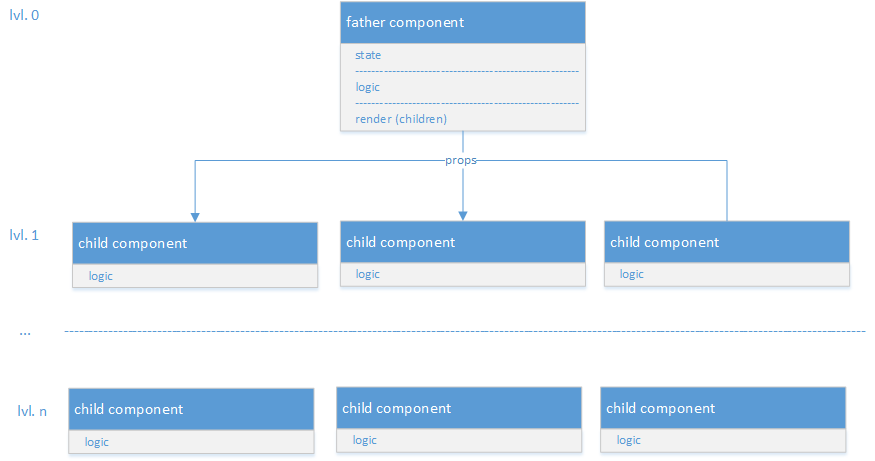
\includegraphics[scale=0.5]{figures/father-children.png}
    \caption{Επικοινωνία μεταξύ πατέρα-παιδιών.}
    \label{fatherchild}
\end{figure}

\subsubsection{\tl{WelcomeScreen}}
Σκοπός της οθόνης έναρξης της εφαρμογής είναι να καλωσορίσει το χρήστη με ένα σύντομο και φιλικό μήνυμα. Η \tl{WelcomeScreen} παίζει καθοριστικό ρόλο στην πρώτη εντύπωση του χρήστη.  Για το λόγο αυτό, θα πρέπει να δωθεί ιδιαίτερη σημασία στα στοιχεία που θα χρησιμοποιηθούν σε αυτό το σημείο της εφαρμογής. Χωρίς πολλές πληροφορίες, ο χρήστης εισάγεται στο νόημα της εφαρμογής και παροτρύνεται να ξεκινήσει να τη χρησιμοποιεί. \newline
\indent
Ένα εξίσου σημαντικό στοιχείο που πρέπει να ληφθεί υπόψη είναι η χρονική απόσταση μεταξύ \tl{WelcomeScreen} και \tl{HomeScreen}. Στην περίπτωση όπου η έναρξη αποτελεί μια πολυσέλιδη εισαγωγική διαδικασία, με αρκετά κείμενα, είναι πολύ πιθανό να αποθαρρυνει το χρήστη. Ο χρόνος που απαιτείται για να μεταβεί ο χρήστης από την οθόνη έναρξης στην κεντρική οθόνη της εφαρμογής πρέπει να είναι ο ελάχιστος δυνατός. Οι μόνοι παράγοντες από τους οποίους θα εξαρτηθεί αυτό, είναι η διαδικασία εγγραφής του χρήστη στην εφαρμογή και οι απαραίτητες ειδοποιήσεις που σχετίζονται με εξωτερικές ρυθμίσεις της συσκευής για την εύρυθμη και ολοκληρωμένη λειτουργία της εφαρμογής. \newline
\indent
Είναι πολύ συχνό το φαινόμενο διαγραφής μιας εφαρμογής πρωτού ο χρήστης φτάσει στην κεντρική οθόνη. Αυτό οφείλεται κατά κύριο λόγο στα πολλαπλά μηνύματα που εμφανίζονται κατά τη διαδιασία εισόδου στην εφαρμογή. Συνεχόμενες ειδοποιήσεις σχετικές με ρυθμίσεις που απαιτούνται εντός της εφαρμογής κουράζουν το χρήστη και απομακρύνουν την εφαρμογή από το στόχο της, να κερδίσει δηλαδή το ενδιαφέρον του χρήστη. οι ειδοποιήσεις θα πρέπει να βρίσκονται σε λογικά σημεία στην εφαρμογή και να εμφανίζονται μόνο όταν ο χρήστης πρόκειται να χρησιμοποιήσει μια υπηρεσία που απαιτεί εξωτερικούς πόρους και πρόκειται να αλλάξει τις ρυθμίσεις της συσκευής.


\subsubsection{\tl{RegistrerScreen}}
Η οθόνη εγγραφής του χρήστη στην εφαρμογή είναι ένα ιδιαίτερα κρίσιμο σημείο της εφαρμογής. Ο χρήστης σχηματίζει την πρώτη του εντύπωση και για το λόγο αυτό θα πρέπει η οθόνη εγγραφής να μην εμποδίζει τη διαμόρφωση μιας θετικής εικόνας. Αυτό σημαίνει πως θα πρέπει να είναι φιλική όσον αφορά στη χρήση της, να μην αποτελείται από κουραστικά στοιχεία και περιττές λεπτομέρειες και να είναι σύντομη. Στο σχεδιασμό της φόρμας εγγραφής θα πρέπει να ληφθεί υπόψη το γεγονός ότι ο χρήστης δεν αντιδρά θετικά στις καθυστερήσεις και τις πρόσθετες υποχρεώσεις που δημιουργεί η διαδικσία εγγραφής στην εφαρμογή. Έτσι, ο χρόνος που απαιτείται για τη συμπλήρωση της φόρμας και την ολοκλήρωση της διαδικασίας εγγραφής θα πρέπει να είναι ο ελάχιστος δυνατός. \newline
\indent
Συνεπώς, η οθόνη θα περιέχει μόνο τα απαραίτητα στοιχεία για την σωστή εγγραφή του χρήστη στην εφαρμογή. Η φόρμα εγγραφής θα είναι σύντομη αλλά επεξημηματική, τα στοιχεία εισόδου θα είναι λιτά αλλά ευδιάκριτα και το πλήκτρο υποβολής θα είναι κατάλληλου μεγέθους και εύκολο στη χρήση. Κάθε στοιχείο εισόδου θα αντιστοιχίζεται με την κατάλληλη μορφή του πληκτρολογίου, ανάλογα με τη φύση του. Δηλαδή, εάν η είσοδος απαιτεί ηλεκτρονική διεύθυνση, τότε το πληκτρολόγιο θα πααρέχει γρήγορη πρόσβαση στα απαραίτητα σύμβολα και αλφαριθμητικούς χαρακτήρες που απαιτούνται στην περίπτωση αυτή. Ο κωδικός πρόσβασης θα προστατεύεται αυτόματα και για λόγους αποφυγής προβλημάτων θα ζητείται η επιβεβαίωσή του. \newline 
\indent
Στην περίπτωση όπου υπάρχουν σφάλματα, μια διεπαφή σφαλμάτων θα εμφανίζει κατάλληλα μηνύματα λάθους στο χρήστη. Τα μηνύματα θα είναι σύντομα και σαφή και θα στοχεύουν κάθε λάθος ξεχωριστά για την καλύτερη αντιμετώπισή τους από την πλευρά του χρήστη. Με αυτό τον τρόπο, επιδιώκεται η γρήγορη και αποτελεσματική συμπλήρωση της φόρμας και η μετάβαση στο κύριο τμήμα της εφαρμογής.


\subsubsection{\tl{LoginScreen}}
Η οθόνη σύνδεσης είναι πολύ πιο απλή από την οθόνη εγγραφής και έχει σκοπό την γρήγορη είσοδο του χρήστη στην εφαρμογή. Για το λόγο αυτό, περιέχει μόνο τις εισόδους για τα διαπιστευτήρια του χρήστη. Ο χρήστης στη φόρμα σύνδεσης καλείται να παραθέσει το συνδυασμό ηλεκτρονικής διεύθυνσης και κωδικού πρόσβασης. Στην περίπτωση που ο παραπάνω συνδυασμός δεν είναι σωστός, η φόρμα ανταποκρίνεται με κατάλληλο μήνυμα λάθους, μέσω μιας διεπαφής σφαλμάτων παρόμοια με αυτή της φόρμας εγγραφής.

\begin{figure}[H]
    \centering
    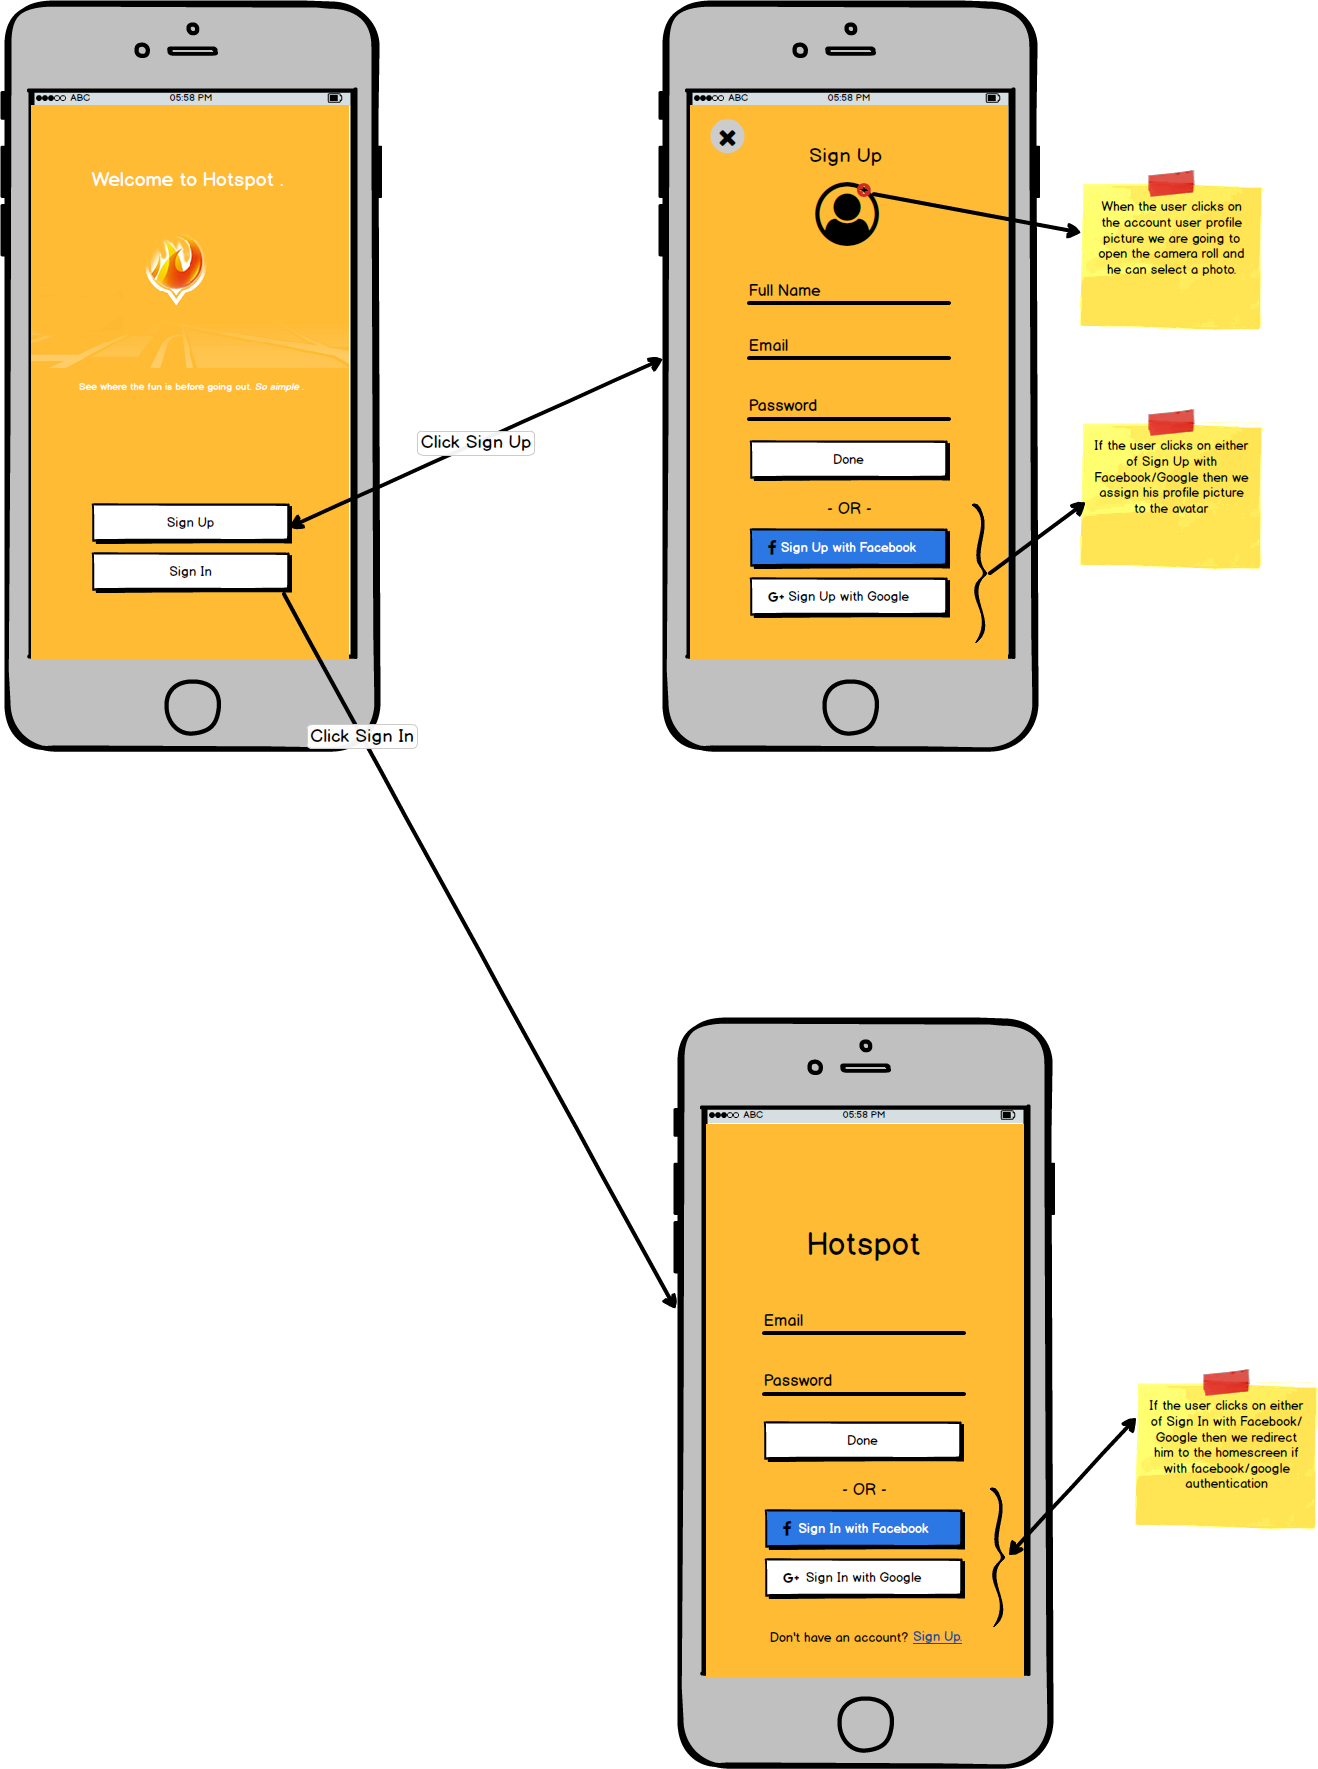
\includegraphics[scale=0.23]{figures/sign-up-sign-in.png}
    \caption{Αρχικό σχέδιο της οθόνης έναρξης και των οθονών εγγραφής/σύνδεσης.}
    \label{authmockup}
\end{figure}

\subsubsection{\tl{HomeScreen}}
Η κεντρική οθόνη αποτελεί τον πυρήνα της εφαρμογής. Για το λόγο αυτό, επιβάλλεται η σχεδίασή της να είναι σφαιρική. Αυτό σημαίνει πως ο χρήστης θα πρέπει να μπορεί να αποκτήσει πρόσβαση σε όλες τις υπόλοιπες οθόνες από το σημείο αυτό. Οι περισσότερες λειτουργικότητες ξεκινούν από την οθόνη αυτή, πράγμα που καθιστά την απόκτηση εμπειρίας από την πλευρά του χρήστη εύκολη και άμεση. \newline

\begin{figure}[H]
    \centering
    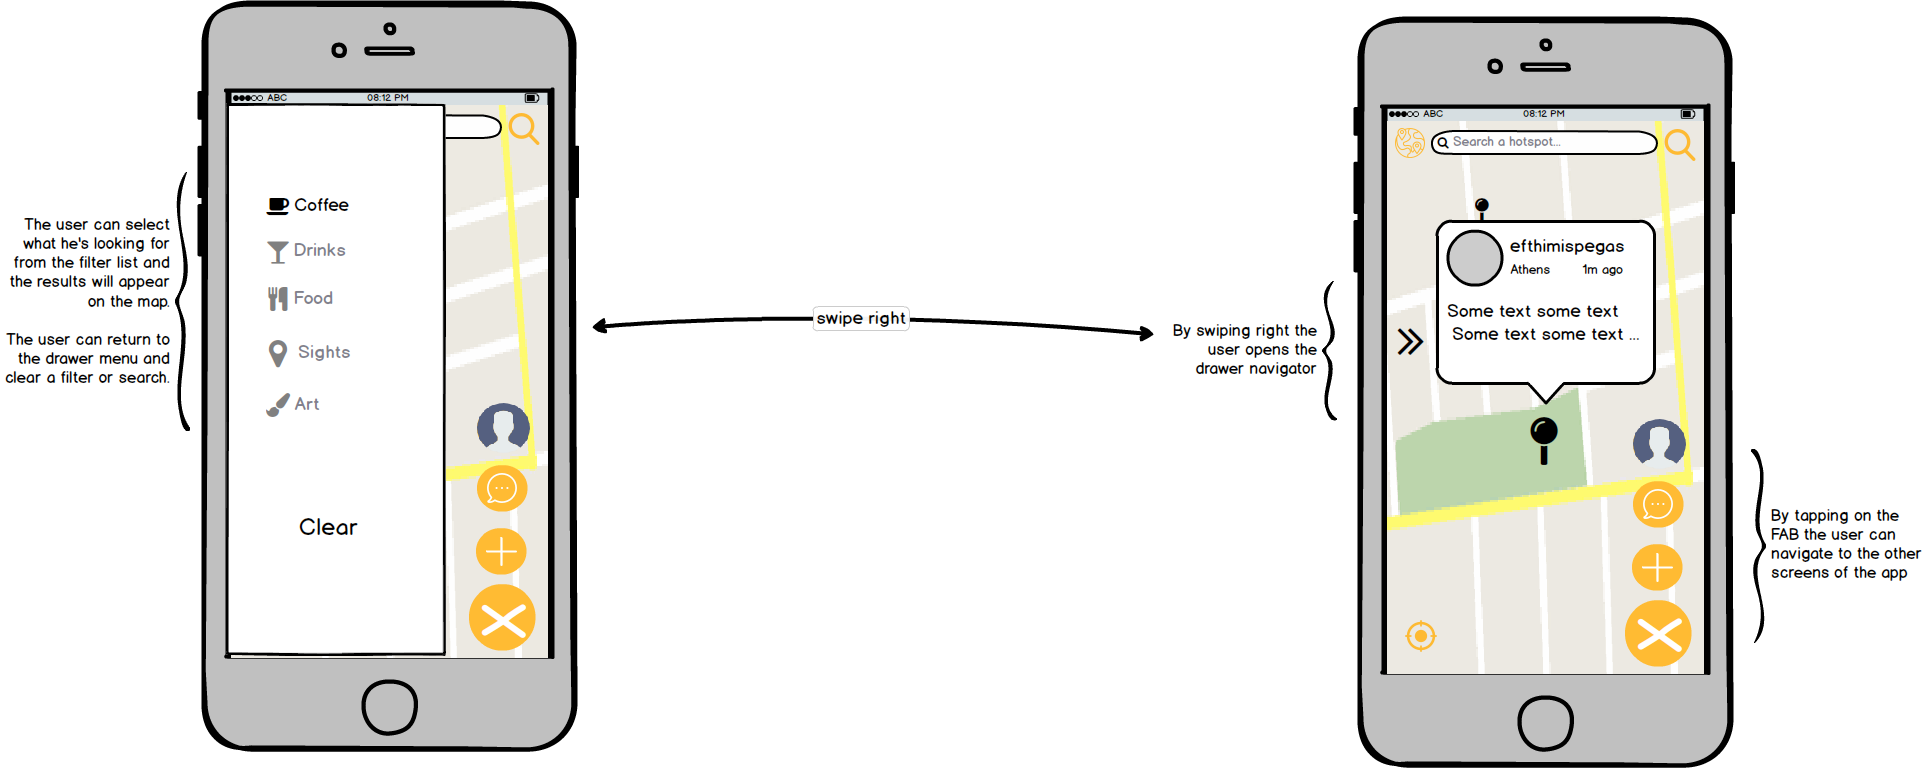
\includegraphics[scale=0.25]{figures/home.png}
    \caption{Αρχικό σχέδιο της κεντρικής οθόνης.}
    \label{homemockup}
\end{figure}

\indent
Η \tl{HomeScreen} περιέχει περισσότερες λειτουργικότητες από κάθε άλλη οθόνη. Προκειμένου ο χρήστης να μπορεί να πλοηγηθεί στις υπόλοιπες οθόνες, θα διαθέτει ένα διακριτικό αλλά κομψό πλήκτρο στο κάτω δεξιά μέρος της οθόνης. Με το πάτημά του θα αναδύονται επιμέρους πλήκτρα με εικονίδια που αντιστοιχούν στις υπόλοιπες οθόνες της εφαρμογής. Για την αναζήτηση συγκεκτριμένων σημείων ενδιαφέροντος, ο χρήστης θα εισάγει τις λέξεις-κλειδιά στην μπάρα αναζήτησης στο πάνω μέρος της οθόνης και έπειτα θα μπορεί είτε να επιλέξει ένα απο τα προτεινόμενα αποτελέσματα, είτε να κάνει γενικευμένη αναζήτηση μέσω του πλήκτρου αναζήτησης. Επιπρόσθετα φίλτρα αναζήτησης θα εμφανίζονται όταν ο χρήστης σύρει το αριστερό άκρο της οθόνης προς τα δεξιά, ή πατάει στο εικονίιδο που βρίσκεται στο επάνω αριστερά μέρος της οθόνης. Προηγούμενες αναζητήσεις ή εφαρμοσμένα φίλτρα θα αναιρούνται επιλέγοντας το πλήκτρο καθαρισμού από το ίδιο μενού. Τέλος, ο χρήστης θα μπορεί αν επαναφέρει τη θέση του χάρτη στην τοποθεσία του μέσω πλήκτρου για το σκοπό αυτό που θα βρίσκεται στο κάτω αριστερά μέρος της οθόνης. 
\newline
\indent
Από τα παραπάνω γίνεται αντιληπτή η αυξημένη πολυπλοκότητα που συνοδεύει τη σχεδίαση της \tl{HomeScreen}. Ωστόσο, είναι κρίσιμο ο χρήστης να μην οδηγείται σε αυτό το συμπέρασμα κατά τη χρήση. Κάθε βήμα στη σχεδίαση καθεμιάς από τις προαναφερθείσες λειτουργικότητες θα πρέπει λοιπόν να χαρακτηρίζεται από απλότητα και να είναι βέλτιστη. Αυτό επιτυγχάνεται με τη χρήση απλών και ευδιάκριτων εικονιδίων, την προκαταβολική εκτέλεση πολλαπλών λειτουργιών σε προηγούμενο χρόνικό σημείο και την υλοποίηση κάθε διεπαφής με εξελιγμένες βιβλιοθήκες και εργαλεία που χρησιμοποιούνται από τις πιο καταξιωμένες εφαρμογές σήμερα. Με αυτό τον τρόπο, δίνεται στο χρήστη η εντύπωση της αποδοτικής και ομαλής λειτουργίας της εφαρμογής, πράγμα που αποτελεί και τον τελικό στόχο.


\subsubsection{\tl{CreateHotspotScreen}}

\begin{figure}[h]
    \centering
    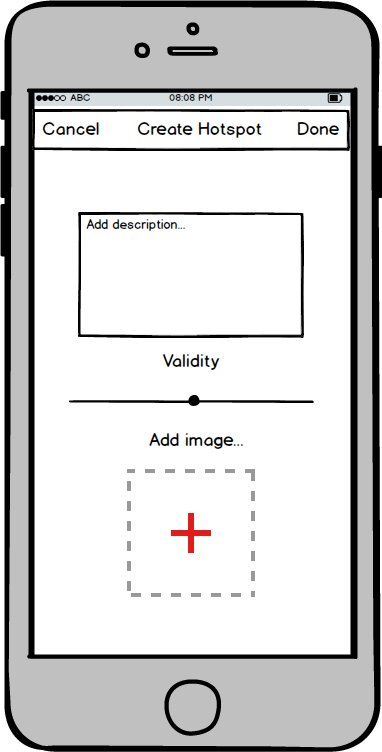
\includegraphics[scale=0.25]{figures/create-hotspot.png}
    \caption{Αρχικό σχέδιο της οθόνης δημιουργίας νέου \tl{hotspot}.}
    \label{createmockup}
\end{figure}

Όταν ο χρήστης θέλει να δημιουργήσει ένα νέο \tl{hotspot}, μπορεί να το κάνει πηγαίνοντας στην \tl{CreateHotspotScreen}. Η οθόνη δημιουργίας νέου \tl{hotspot} εξυπηρετεί έναν αποκλειστικό σκοπό. Για το λόγο αυτό, στη σχεδίασή της συμπεριλήφθησαν στοιχεία που αφορούν στις ανάγκες της συγκεκριμένης οθόνης.
\newline
\indent
Οι προϋποθέσεις που πρέπει να πληροί η οθόνη για να είναι πλήρως λειτουργική και να συναντάει όλες τις απαιτήσεις, είναι η φόρμα δημιουργίας νέου \tl{hotspot}, η διεπαφή για την ενσωμάτωση αρχείου εικόνας και τα βασικά πλήκτρα ενεργειών και πλοήγησης. Η φόρμα είναι βρίσκεται σε απλουστευμένη μορφή και αποτελείται από ένα στοιχείο εισόδου που αντιστοιχεί στην περιγραφή του \tl{hotspot} προς δημιουργία, και ένα \tl{slider} που αντιστοιχεί στο χρονικό διαστημα για το οποίο θα είναι έγκυρο το \tl{hotspot}.
\newline
\indent
Όπως και κάθε οθόνη που δέχεται είσοδο από το χρήστη, έτσι και εδώ, απαιτείται κατάλληλος έλεγχος. Η είσοδος του χρήστη θα συνοδεύεται από διεπαφή μηνυμάτων κατάλληλης μορφής. Στην περίπτωση λάθους, η διεπαφή μηνυμάτων θα εμφανίζει στο χρήστη επεξηγηματικό μήνυμα λάθους, που θα προσδιορίζει το σημείο και το είδος του σφάλματος που έχει δημιουργηθεί. Εάν δεν υπάρχουν σφάλματα, τότε η υποβολή του νέου \tl{hotspot} γίνεται με επιτυχία, και ο χρήστης επαναφέρεται στο χάρτη. Το καινούριο \tl{hotspot} φαίνεται στο χάρτη, στην τοποθεσία του χρήστη.


\subsubsection{\tl{HotspotListScreen}}
Προκειμένου να γίνει περισσότερο λειτουργική, η εφαρμογή ταξινομεί τα προσωπικά \tl{hotspots} του χρήστη. Πηγαίνοντας στη \tl{HotspotListScreen}, ο χρήστης μπορεί να εξευρευνήσει τη λίστα με όλες τις δημοσιεύσεις του. Σε αυτή την οθόνη ο χρήστης μπορεί να διαχειριστεί τα προσωπικά του \tl{hotspots} σε μόλις λίγα βήματα. Σύροντας την οθόνη προς τα επάνω, ο χρήστης μπορεί να περιηγηθεί στη σελίδα και να δει περισσότερα \tl{hotspots}, καθώς και σχετικές πληροφορίες. Η λίστα είναι ταξινομημένη με βάση την ημερομηνία δημιουργίας. Έτσι, το πιο πρόσφατο \tl{hotspot} βρίσκται στην κορυφή, ενώ το παλαιότερο βρίσκεται στο τέλος της λίστας. Επίσης, για την γρηγορότερη φόρτωση και εμφάνιση των δεδομένων της οθόνης, η εφαρμογή φορτώνει τα πρώτα επτά \tl{hotspots} του χρήστη. Έπειτα, ο χρήστης μπορεί να σύρει την οθόνη προς τα επάνω και να πατήσει το πλήκτρο εμφάνισης περισσότερων αποτελεμάτων με την επιγραφή  ``\textit{\tl{show more}}''.

\begin{figure}[H]
    \centering
    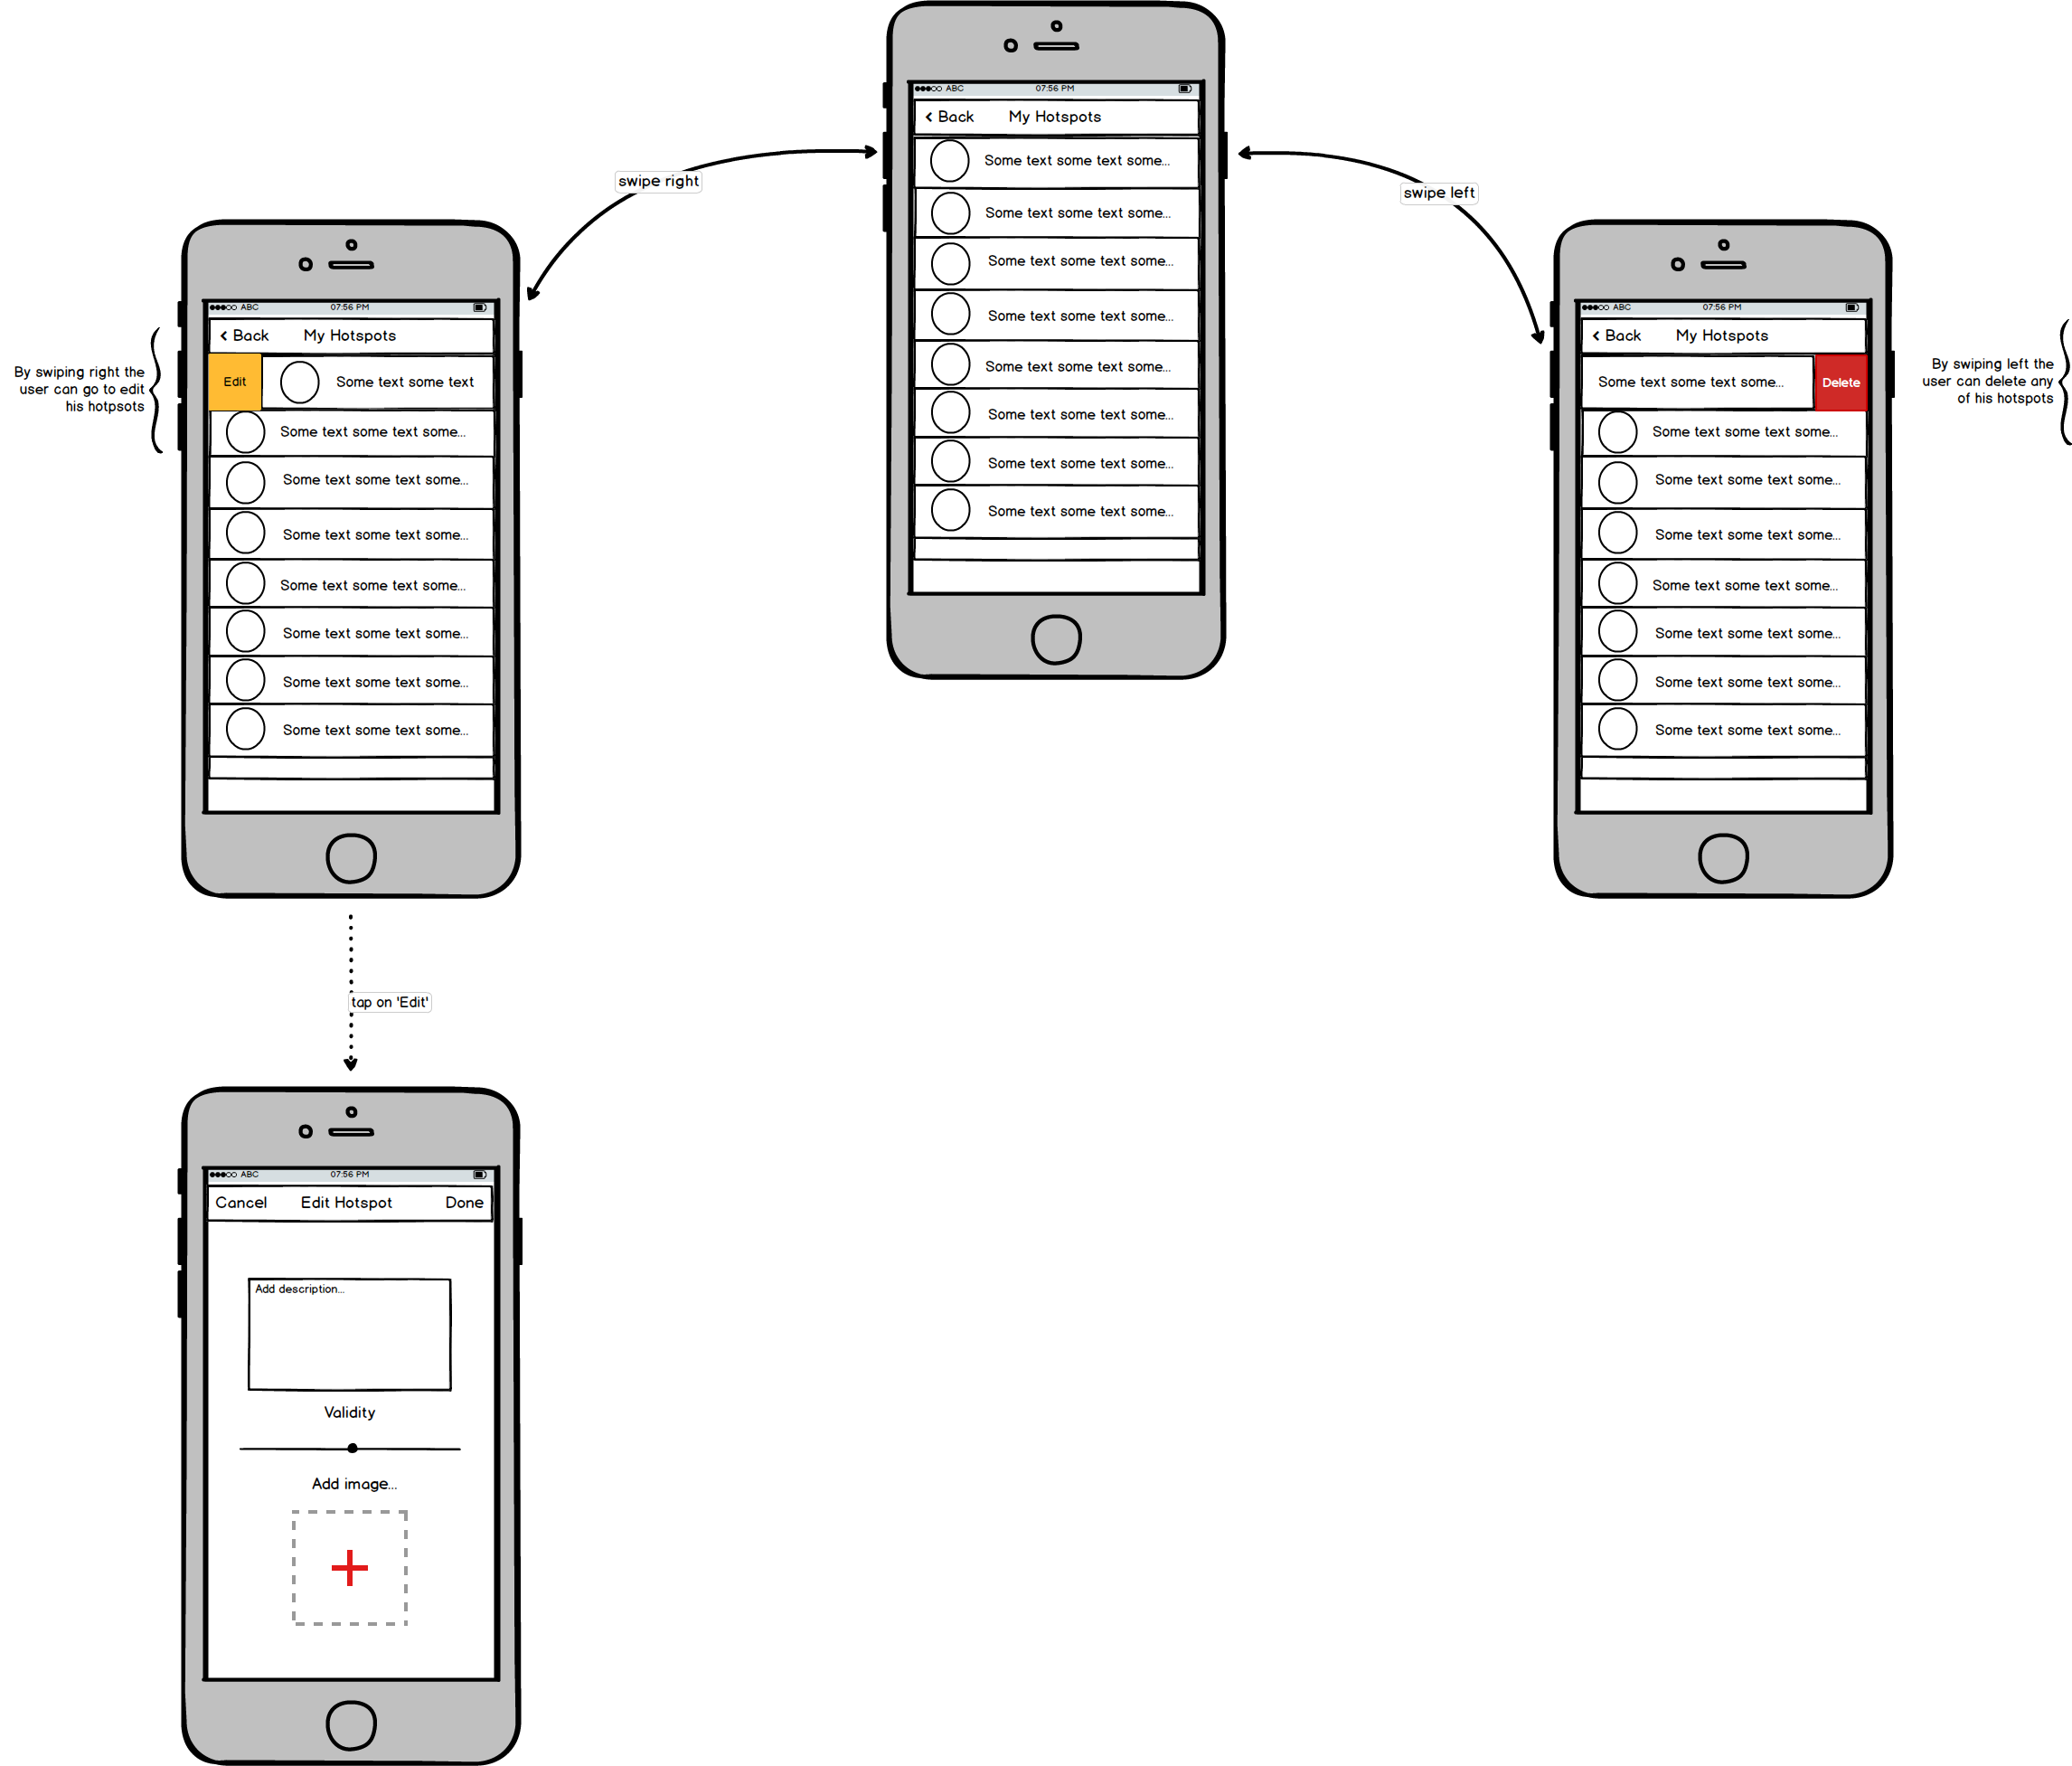
\includegraphics[scale=0.22]{figures/my-hotspots.png}
    \caption{Αρχικό σχέδιο της οθόνης προσωπικών \tl{hotspots} του χρήστη.}
    \label{myhotspotsmockup}
\end{figure}

Στην οθόνη προσωπικών \tl{hotspots}, Ο χρήστης έχει τη δυνατότητα να πραγματοποιήσει αλλαγές στα δικά του \tl{hotspots}. Η λίστα είναι εφοδιασμένη με κρυφές λειτουργικότητες τις οποίες μπορεί να αξιοποιήσει ο χρήστης σύροντας ένα στοιχείο της λίστας προς μια οριζόντια κατεύθυνση. Για την επεξεργασία ενός \tl{hotspot}, ο χρήστης σύρει ένα \tl{hotspot} προς τα δεξιά. Τότε, πατώντας το πλήκτρο επεξεργασίας με την επιγραφή ``\textit{\tl{edit}}'', η εφαρμογή μεταφέρει το χρήστη στη σελίδα επεξεργασίας του επιλεγμένου \tl{hotspot}. Εκεί, ο χρήστης μπορεί να πραγματοποιήσει τις επιθυμητές αλλαγές στην περιγραφή ή την εικόνα του \tl{hotspot}. Για την διαγραφή ενός \tl{hotspot}, ο χρήστης σύρει ένα \tl{hotspot} προς τα αριστερά. Τότε, πατώντας το πλήκτρο διαγραφής με τo εικονίδιο ``\textit{\tl{delete}}'', η εφαρμογή διαγράφει το επιλεγμένο \tl{hotspot} από τη λίστα. \newline
\indent
Η \tl{HotspotListScreen} εξυπηρετεί την ανάγκη του χρήστη να ελέγχει την κατάσταση των προσωπικών του \tl{hotspots}. Είναι σχεδιασμένη έτσι ώστε να παρέχει στο χρήστη τις επιθυμητές πληροφορίες για τα \tl{hotspots} του, χωρίς να χρειάζεται να μεταβεί σε άλλη σελίδα. Για παράδειγμα, μπορεί γρήγορα να δει τον αριθμό των \tl{views} και των \tl{comments} ενός \tl{hotspot}. Εάν ο χρήστης επιθυμεί να δεί αναλυτικές πληροφορίες για ένα συγκεκριμένο \tl{hotspot}, τότε μπορεί να πατήσει στο εικονίδιο σχολίων με την επιγραφή ``\textit{\tl{comments}}''. Στη συνέχεια, η εφαρμογή μεταβαίνει στην οθόνη σχολίων \tl{CommentScreen} του επιλεγμένου \tl{hotspot}. Περισσότερα για την οθόνη αυτή αναφέρονται στην επόμενη παράγραφο.

\subsubsection{\tl{CommentScreen}}
Για μια πιο λεπτομερή περιήγηση στις πληροφορίες σχετικά με κάποιο \tl{hotspot}, ο χρήστης μπορεί να μεταβεί στην \tl{CommentScreen}. Εκεί βρίσκονται όλα τα δεδομένα που αφορούν ένα συγκεκριμένο \tl{hotspot}, όπως ο αριθμός των \tl{comments} και των \tl{views}, σχόλια άλλων χρηστών στο συγκεκριμένο \tl{hotspot}, απαντήσεις πάνω σε σχόλια και φωτογραφία του \tl{hotspot}, αν υπάρχει. \newline
\indent
Η οθόνη αυτή συμπεριλαμβάνει όλα εκείνα τα στοιχεία που έχουν να κάνουν με την αλληλεπίδραση των χρηστών με ένα συγκεκριμένο \tl{hotspot}. Εάν ο χρήστης επιθυμεί να γράψει ένα σχολιασμό ή να απαντήσει σε κάποιο σχόλιο, μπορεί να το κάνει εδώ. Σύροντας την οθόνη προς τα επάνω, ο χρήστης μπορεί χειροκίνητα να μεταφερθεί στο τέλος της λίστας με τα σχόλια, όπου βρίσκεται η διεπαφή δημιουργίας νέου σχολίου. Ένας άλλος τρόπος να επιτευχθεί αυτό είναι σύροντας κάποιο σχόλιο προς τα αριστερά και πατώντας στο πλήκτρο ``\textit{\tl{reply}}''. Η εφαρμογή τότε θα μεταφέρει αυτομάτως το χρήστη στη διεπαφή δημιουργίας νέου σχολίου. Η διεπαφή είναι σχεδιασμένη ώστε να είναι ευδιάκριτη και μοντέρνα, αλλά ταυτοχρόνως απλή. Το τμήμα δημιουργίας νέου σχολίου συνοδεύεται και από το πλήκτρο υποβολής του νέου σχολίου, το οποίο φέρει το χαρακτηριστικό εικονίδιο ``\textit{\tl{send}}''.
\newline
\indent
Η οθόνη είναι σχεδιασμένη ώστε να είναι αποδοτική και γρήγορη. Η λίστα με τα σχόλια θα πρέπει να φορτώνεται άμεσα. Η εμπειρία που προσφέρεται στο χρήστη θα πρέπει να είναι η κα΄λυτερη δυνατή. Συνεπώς, η καθυστέρηση φόρτωσης θα πρέπει να είναι η ελάχιστη δυνατή. Η οθόνη είναι σχεδιαμένη με τέτοιο τρόπο, ώστε αν η λίστα με τα σχόλια είναι αρκετά μεγάλη, τότε να φορτώνεται μόνο ένας ορισμένος αριθμός σχολίων την πρώτη φορά. Εάν ο χρήστης επιθυμεί αν φορτώσει περισσότερα σχόλια, τότε μπορεί να περιηγηθεί στο τέλος της λίστας σύροντας την οθόνη προς τα επάνω και να πατήσει το πλήκτρο με την επιγραφή ``\textit{\tl{load more}}''. Με την τμηματοποίηση της λίστας σχολίων, αποφεύγεται η περίπτωση μεγάλης καθυστέρησης φόρτωσης λόγω τεράστιου όγκου δεδομένων.


\begin{figure}[H]
    \centering
    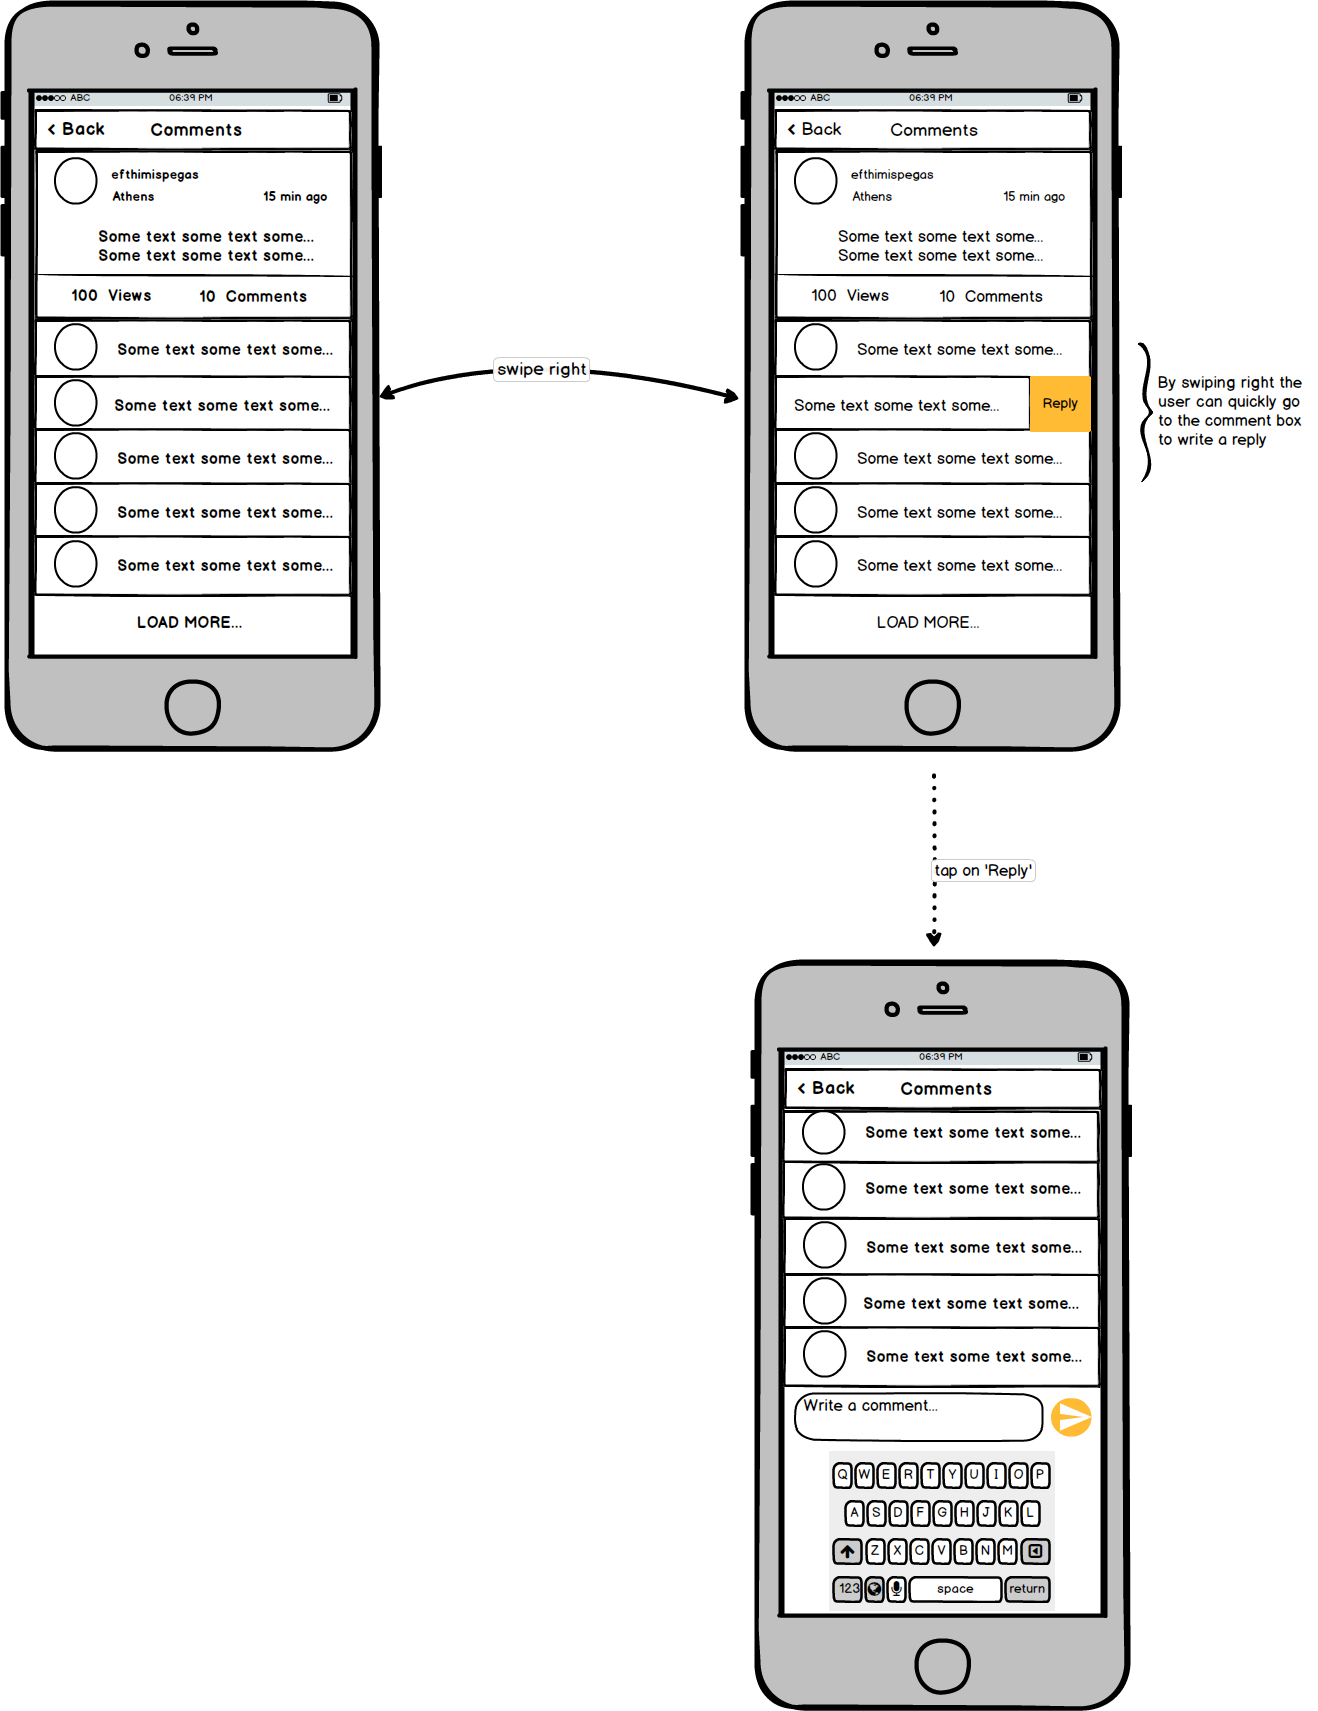
\includegraphics[scale=0.25]{figures/comments.png}
    \caption{Αρχικό σχέδιο της οθόνης σχολιασμών επάνω σε κάποιο \tl{hotspot}.}
    \label{commentmockup}
\end{figure}



\subsubsection{\tl{ProfileScreen}}
Ο προσωπικός λογαριασμός του χρήστη είναι ένα κρίσιμο σημείο της εφαρμογής και έχει δωθεί ιδιαίτερη προσοχή στη σχεδίασή του. Ο χρήστης θα πρέπει να μπορεί, από τη μία να προβάλλει τα προσωπικά του στοιχεία και από την άλλη να επεξεργαστεί τις προσωπικές του ρυθμίσεις ή να αλλάξει το \tl{profile} του. Εδώ ο χρήστης μπορεί να δει επίσης δεδομένα χρήσης της εφαρμογής, όπως ποσοστά αλληλεπίδρασης με άλλους χρήστες, συνολικό αριθμό σχολίων και προβολών, καθώς επίσης και το είδος του κοινού με το οποίο ο χρήστης αλληλεπιδρά περισσότερο. Στόχος της οθόνης \tl{profile} είναι να ολοκληρώσει τη θετική εικόνα του χρήστη για την εφαρμογή και να αυξήσει το ενδιαφέρον του για αυτή.

\begin{figure}[H]
    \centering
    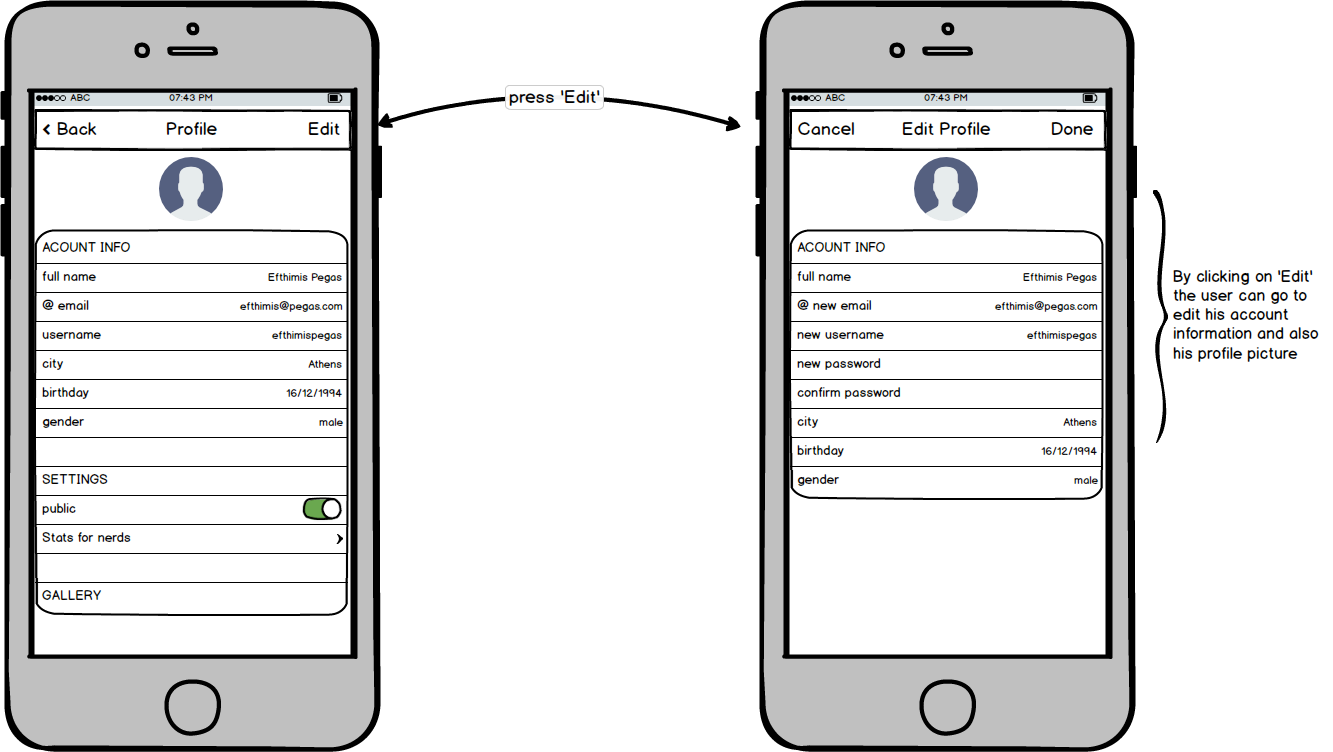
\includegraphics[scale=0.25]{figures/profile.png}
    \caption{Αρχικό σχέδιο της οθόνης προσωπικού λογαριασμού του χρήστη.}
    \label{profilemockup}
\end{figure}


Οι πληροφορίες που προβάλλονται στην \tl{ProfileScreen} διακρίνονται σε τρεις κατηγορίες. Ταξινομημένα πρώτα είναι τα προσωπικά στοιχεία του χρήστη, με τα οποία συπλήρωσε τη φόρμα εγγραφής την πρώτη φορά που εισήλθε στην εφαρμογή. Έπειτα ακολουθούνε οι προσωπικές ρυθμίσεις του χρήστη, όπως το είδος του λογαριασμού που έχει δημιουργήσει (\tl{public} ή \tl{private}). Εάν ο χρήστης το επιθυμεί, μπορεί να προβάλλει τα στατιστικά δεδομένα που βρίσκονται σε ξεχωριστή σελίδα, πατώντας το βέλος που βρίσκεται στα δεξιά της επιγραφής ``\textit{\tl{Stats for nerds}}''. Τέλος, στο κάτω μέρος της οθόνης βρίσκεται η συλλογή φωτογραφιών του χρήστη από τα προσωπικά \tl{hotspots} που έχει δημιουργήσει ο ίδιος στο παρελθόν.
\newline
\indent
Για την επεξεργασία των προσωπικών του στοιχείων, ο χρήστης μπορεί να μεταβεί στην σελίδα επεξεργασίας \tl{profile}. Πατώντας το πλήκτρο με την επιγραφή ``\textit{\tl{Edit}}'' που βρίσκεται στο δεξί μέρος της επικεφαλίδας, ο χρήστης μεταφέρεται στην \tl{EditProfileScreen}. Εκεί, ο χρήστης μπορεί να επεξεργαστεί τα προσωπικά του στοιχεία, όπως το όνοματεπώνυμό του, την ηλεκτρονική του διεύθυνση, το όνομα χρήστη του, την εικόνα προφίλ του κλπ. Ακόμη, είναι εφικτή η αλλαγή των ρυθμίσεων του χρήστη, όπως το είδος του λογαριασμού. Για την επιτυχή αλλαγή των στοιχείων του ο χρήστης πρέπει να συμπληρώσει τον κωδικό πρόσβασης. Η φόρμα επεξεργασίας των προσωπικών δεδομέων του χρήστη συνοδεύεται από μια διεπαφή μηνυμάτων λάθους, όπως και κάθε οθόνη που απαιτεί είσοδο από το χρήστη. Στην περίπτωση όπου ένα ή περισσότερα πεδία είναι εσφαλμένα, κατάλληλο μήνυμα λάθους εμφανίζεται κάτω από το αντίστοιχο πεδίο. Στην περίπτωση όπου δεν υπάρχουν σφάλματα, η υποβολή της φόρμας ολοκληρώνεται με επιτυχία και ο χρήστης μεταφέρεται πίσω στον προσωπικό του λογαριασμό. Τα νέα στοιχεία του χρήστη φαίνονται στην οθόνη.
\newline
\indent
Χαρακτηριστικό της εφαρμογής αποτελεί το γεγονός ότι δεν είναι εύκολη η αποσύνδεση του χρήστη από την εφαρμογή. Αυτό οφείλεται στο γεγονός ότι το πλήκτρο αποσύνδεσης δεν υπάρχει σε καμία από τις προηγούμενες οθόνες. Έτσι, ο χρήστης δεν μπορεί να αποσυνδεθεί παρά μόνο όταν έχει ολοκληρώσει την περιήγησή του εντός της εφαρμογής και έχει αποκτήσει μια πλήρη εικόνα των υπηρεσιών που προσφέρει. Για την αποσύνδεση από την εφαρμογή, ο χρήστης μεταβαίνει στον προσωπικό του λογαριασμό και πατάει το πλήκτρο αποσύνδεσης που φέρει την επιγραφή ``\textit{\tl{Log out}}''. Έπειτα, μεταφέρεται αυτόματα στην οθόνη έναρξης της εφαρμογής.
\newline
\indent
Είναι καθήκον της λογικής σχεδίασης της εφαρμογής να ενθαρρύνει συνεχώς την αλληλεπίδραση του χρήστη με τις υπηρεσίες της. Όπως φαίνεται από τα παραπάνω, αυτό επιτυγχάνεται τόσο μέσα από την παροχή πληθώρας λειτουργικοτήτων, όσο και μέσω της παρουσίασης στατιστικών δεδομένων που αφορούν τη σχέση του χρήστη με το υπόλοιπο σύνολο και δημιουργούν μια εικόνα της θέσης του χρήστη εντός του οικοσυστήματος της εφαρμογής. Αυτό συνεισφέρει στη συνεχή δράση του χρήστη και την ανάπτυξη στενών σχέσεων με την εφαρμογή. 



\section{Σχεδίαση Συστήματος Εξυπηρέτησης Αιτημάτων}
Στην προηγούμενη ενότητα καλύφθηκε η λογική που ακολουθήθηκε στη σχεδίαση του \tl{client} της εφαρμογής. Αναλύθηκαν οι δομές που απαρτίζουν τις διάφορες διεπιφάνειες χρήστη, και παρουσιάστηκαν τα αρχικά σχέδια αυτών. Σε αυτή την ενότητα θα αναπτυχθούν οι τεχνικές σχεδίασης του \tl{server} και των υποσυστημάτων του. \newline \indent 
Στην σχεδίαση του εξυπηρετητή αιτημάτων της εφαρμογής, πρωταρχικός σκοπός είναι η αποσύμπλεξη των λειτουργιών που δημιουργεί ένα αίτημα. Κάθε ενέργεια που λαμβάνει χώρα σε μια από τις διεπιφάνειες χρήστη, πυροδοτεί μια σειρά κλήσεων που απαιτούν τη μεταφορά δεδομένων από και προς τον \tl{server}. Ο \tl{server} έχει σχεδιαστεί με τέτοιο τρόπο, ώστε κάθε αίτημα να αποσυναρμολογείται στις επιμέρους διακριτές λειτουργίες που πρέπει να εκτελεστούν. Οι λειτουργίες αυτές δρομολογούνται με τη σειρά τους στα κατάλληλα υποσυστήματα για την εξυπηρέτησή τους.  

\subsection{Λογική Σχεδίασης Εξυπηρετητή και Υποσυστήματα}

\begin{figure}[H]
    \centering
    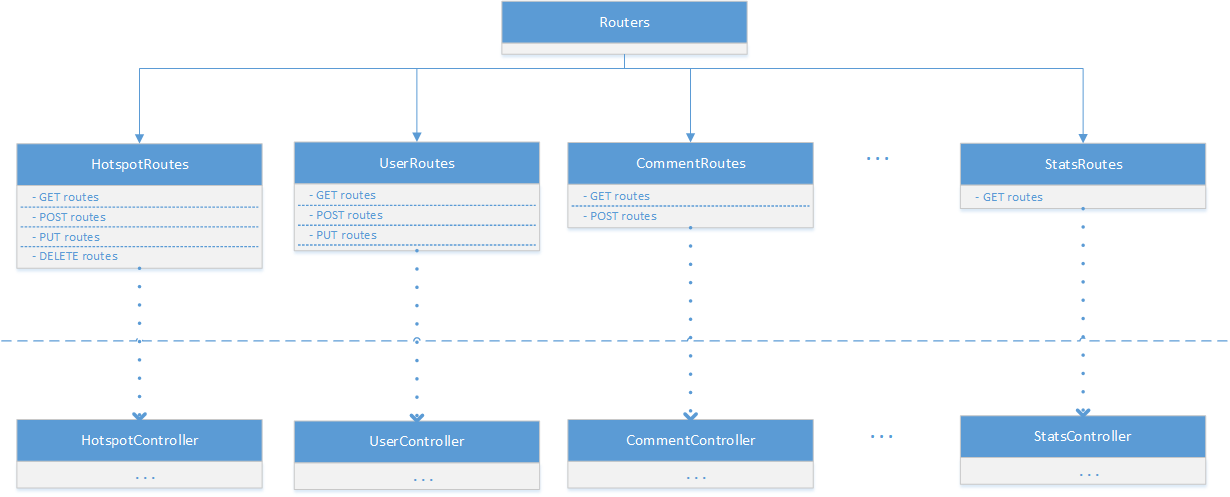
\includegraphics[scale=0.4]{figures/router-system.png}
    \caption{Λογική σχεδίασης του συστήματος δρομολόγησης αιτημάτων.}
    \label{routersystem}
\end{figure}

Ο \tl{server} της εφαρμογής θα συνίσταται από ένα σύστημα ελεγκτών (\tl{controllers}) και δρομολογητών (\tl{routers}), με σκοπό την αποτελεσματική και γρήγορη ικανοποίηση των αιτημάτων που δημιουργεί ο \tl{client}. Κάθε δρομολογητής θα είναι υπεύθυνος για την σωστή ταξινόμηση των αιτημάτων με βάση τη φύση τους και την δρομολόγηση στον κατάλληλο ελεγκτή. Έπειτα, ο ελεγκτής θα εκτελεί μια σειρά λειτουργιών που αντιστοιχούν στο συγκεκριμένο αίτημα που δημιουργήθηκε. Μόλις ολοκληρωθεί η παραπάνω διαδικασία, το αποτέλεσμα επιστρέφεται σε κατάλληλη μορφή πίσω στον \tl{client}.
\newline
\indent
Το σύστημα δρομολόγησης των αιτημάτων διαιρείται σε επιμέρους \tl{routers} (βλ. Σχ. \ref{routersystem}). Για την καλύτερο προγραμματισμό του συστήματος και την απλοποίηση της σχεδίασης, επιλέχθηκε ως κριτήριο διάκρισης η φύση των λειτουργιών που εξυπηρετεί κάθε \tl{route} (περισσότερα στην ενότητα ΠΟΙΑ ΕΝΟΤΗΤΑ).
\newline
\indent
Το σύστημα εξυπηρέτησης των αιτημάτων υλοποιείται από \tl{controllers} που καθορίζουν τις εντολές που θα εκτελεστούν για την ολοκλήρωση κάθε αιτήματος (βλ. Σχ. \ref{controllersystem}). Οι εντολές συνοψίζονται σε μεθόδους, γνωστές ως ελεγκτές. Κάθε ελεγκτής αντιστοιχίζεται στην εξυπηρέτηση ενός αποκλειστικού αιτήματος. Το σύστημα των ελεγκτών είναι σχεδιασμένο ώστε να γίνεται κατανοητό από τον προγραμματιστή και ευέλικτο όσον αφορά στην επεξεργασία του. Όπως και στο σύστημα των δρομολογητών, έτσι και εδώ, κριτήριο στην διακριτοποίηση των ελεγκτών αποτελεί η φύση του αιτήματος (περισσότερα στην ενότητα ΠΟΙΑ ΕΝΟΤΗΤΑ).

\begin{figure}[H]
    \centering
    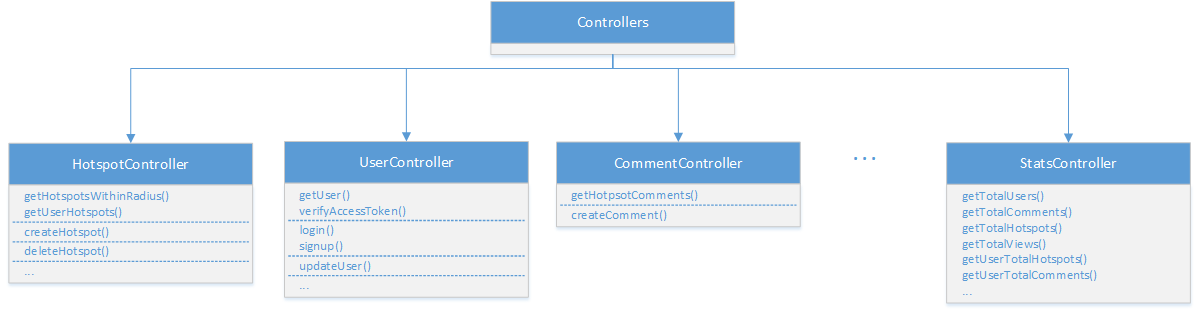
\includegraphics[scale=0.4]{figures/controller-system.png}
    \caption{Λογική σχεδίασης του συστήματος ελεγκτών στον εξυπηρετητή αιτημάτων της εφαρμογής.}
    \label{controllersystem}
\end{figure}

Από τα παραπάνω λοιπόν, γίνεται αντιληπτή η λογική πορεία εξυπηρέτησης αιτημάτων στην οποία βασίζεται ο \tl{server}. Ωστόσο, κατά την πορεία αυτή γίνεται πρόσβαση σε δεδομένα τα οποία είναι αποθηκευμένα σε έναν ειδικά διαμορφωμένο χώρο. Ο αποθηκευτικός αυτός χώρος αποτελεί τη βάση δεδομένων της εφαρμογής και αποτελεί ίσως το σημαντικότερο κομμάτι του \tl{backend}. Στην ενότητα που ακολουθεί θα αναλυθούν οι βασικές σχεδιαστικές τεχνικές που διέπουν τη βάση δεδομένων  της εφαρμογής, καθώς επίσης και τα μοντέλα στα οποία οργανώνονται τα δεδομένα της εφαρμογής.


\section{Σχεδίαση Μοντέλου Βάσης Δεδομένων}
Τα πολλά αιτήματα μεταξύ client-server δημιουργούν την ανάγκη για συνεχείς προσπελάσεις της βάσης δεδομένων. Συνεπώς, η δομή που θα ακολουθεί η βάση θα πρέπει να είναι σχεδιασμένη με τέτοιο τρόπο, ώστε να ευνοεί τη συνεχή πρόσβαση σε αυτή. Για να επιτευχθεί αυτό, θα πρέπει η μοντελοποίηση των δεδομένων να γίνεται με όσο το δυνατόν λιγότερες εξαρτήσεις και με τη χρήση απλών δομών για υψηλή απόδοση. 

\subsection{Μοντελοποίηση Δεδομένων}


\begin{figure}[H]
    \centering
    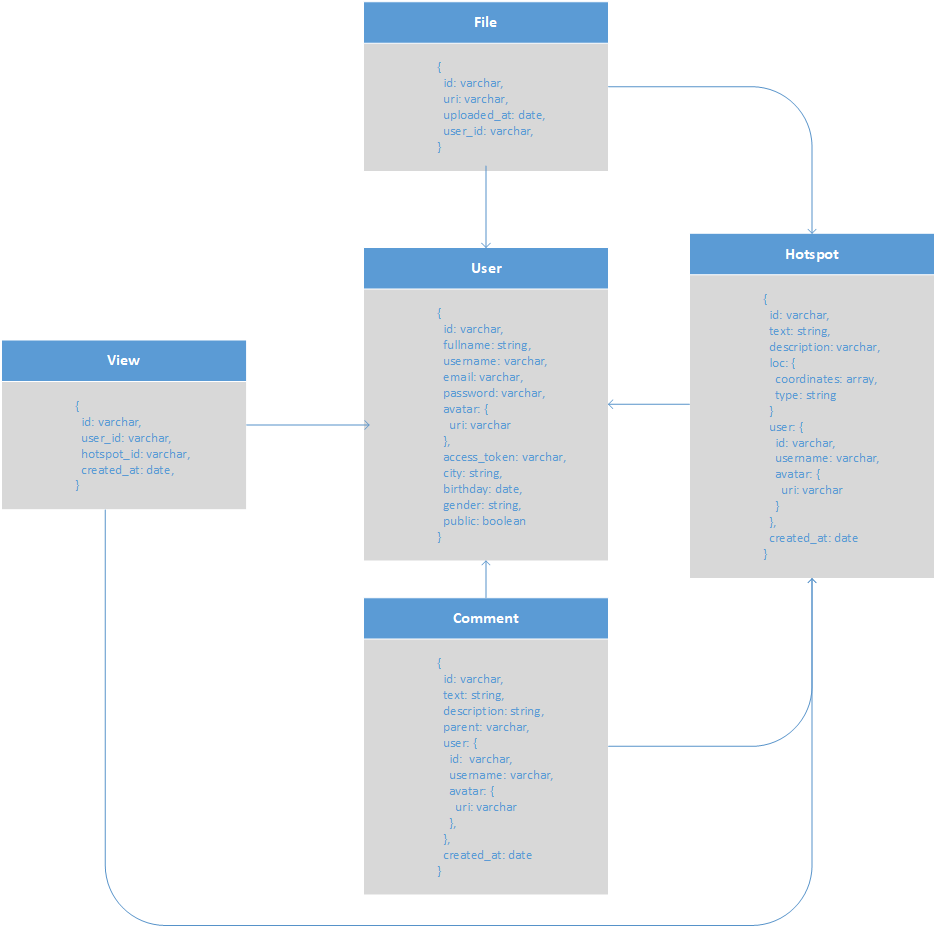
\includegraphics[scale=0.5]{figures/db-models.png}
    \caption{Σχέδιο μοντελοποίσης των δεδομένων της εφαρμογής.}
    \label{dbmodel}
\end{figure}

Όπως αναφέρθηκε στην ενότητα 3.3.2, τα δεδομένα της εφαρμογής μοντελοποιούνται σε \tl{collections}. Η εσωτερική διάρθρωση κάθε τέτοιου μοντέλου περιλαμβάνει ορισμένες ιδιότητες και κάθε μοντέλο που δημιουργείται θα πρέπει να τις ακολουθεί αυστηρά. Κάθε μοντέλο διακρίνεται από τα υπόλοιπα της ίδιας συλλογής μέσω του αναγνωριστικού \tl{ID} το οποίο προσδίδεται αυτόματα σε αυτό. Επίσης, υπάρχει η πιθανότητα κάποια ιδιότητα να είναι μοναδική για κάθε μοντέλο (πχ. η ηλεκτρονική διεύθυνση στο μοντέλο χρήστη). Αυτό επιτυγχάνεται με τον ορισμό ενός δείκτη μοναδικότητας (\tl{uniqueness index}) στην συγκεκριμένη ιδιότητα του μοντέλου. Τα νέα μοντέλα αποθηκεύονται στην αντίστοιχη συλλογή για μετέπειτα χρήση από την εφαρμογή. Στο σχ. \ref{dbmodel} φαίνεται η δομή των μοντέλων της εφαρμογής, καθώς και οι χαρακτηριστικές ιδιότητες του κάθε μοντέλου. 
\newline
\indent
Η αναπαράσταση των δεδομένων με αυτό τον τρόπο, δίνει στον \tl{server} τη δυνατότητα να προσπελαύνει τη βάση δεδομένων με μεγάλη ταχύτητα. Έτσι, η αναζήτηση δεδομένων γίνεται σε μικρό χρονικό διάστημα και η απόδοση της εφαρμογής είναι η βέλτιστη δυνατή. Το ζητούμενο αυτό είναι απότα κυριότερα όταν πρόκειται για την σχεδίαση μιας εφαρμογής με πολλούς χρήστες, μιας και δημιουργούνται συνεχώς αιτήματα για πρόσβαση στη βάση δεδομένων. Η ύπαρξη απλοποιημένων μοντέλων βοηθάει στην γρήγορη εξυπηρέτηση των παραπάνω αιτημάτων και δίνει τη δυνατότητα παραλληλοποίησης των διαδικασιών.
\newline
\indent
Καθοριστικό ρόλο στην ταχύτητα πρόσβασης στη βάση δεδομένων παίζει και η επιλογή της τεχνολογίας. Για το λόγο αυτό έχει επιλεχθεί η \tl{MongoDB} ως το είδος της βάσης που θα χρησιμοποιηθεί στην υλοποίηση. Η \tl{MongoDB} επικεντρώνεται στην εξυπηρέτηση πολλαπλών αιτημάτων που απαιτούν ταυτόχρονη πρόσβαση σε δεδομένα της βάσης, αποτελόντας συνεπώς και την καλύτερη λύση (βλ. σχ. \ref{mondodb}).

\begin{figure}[H]
    \centering
    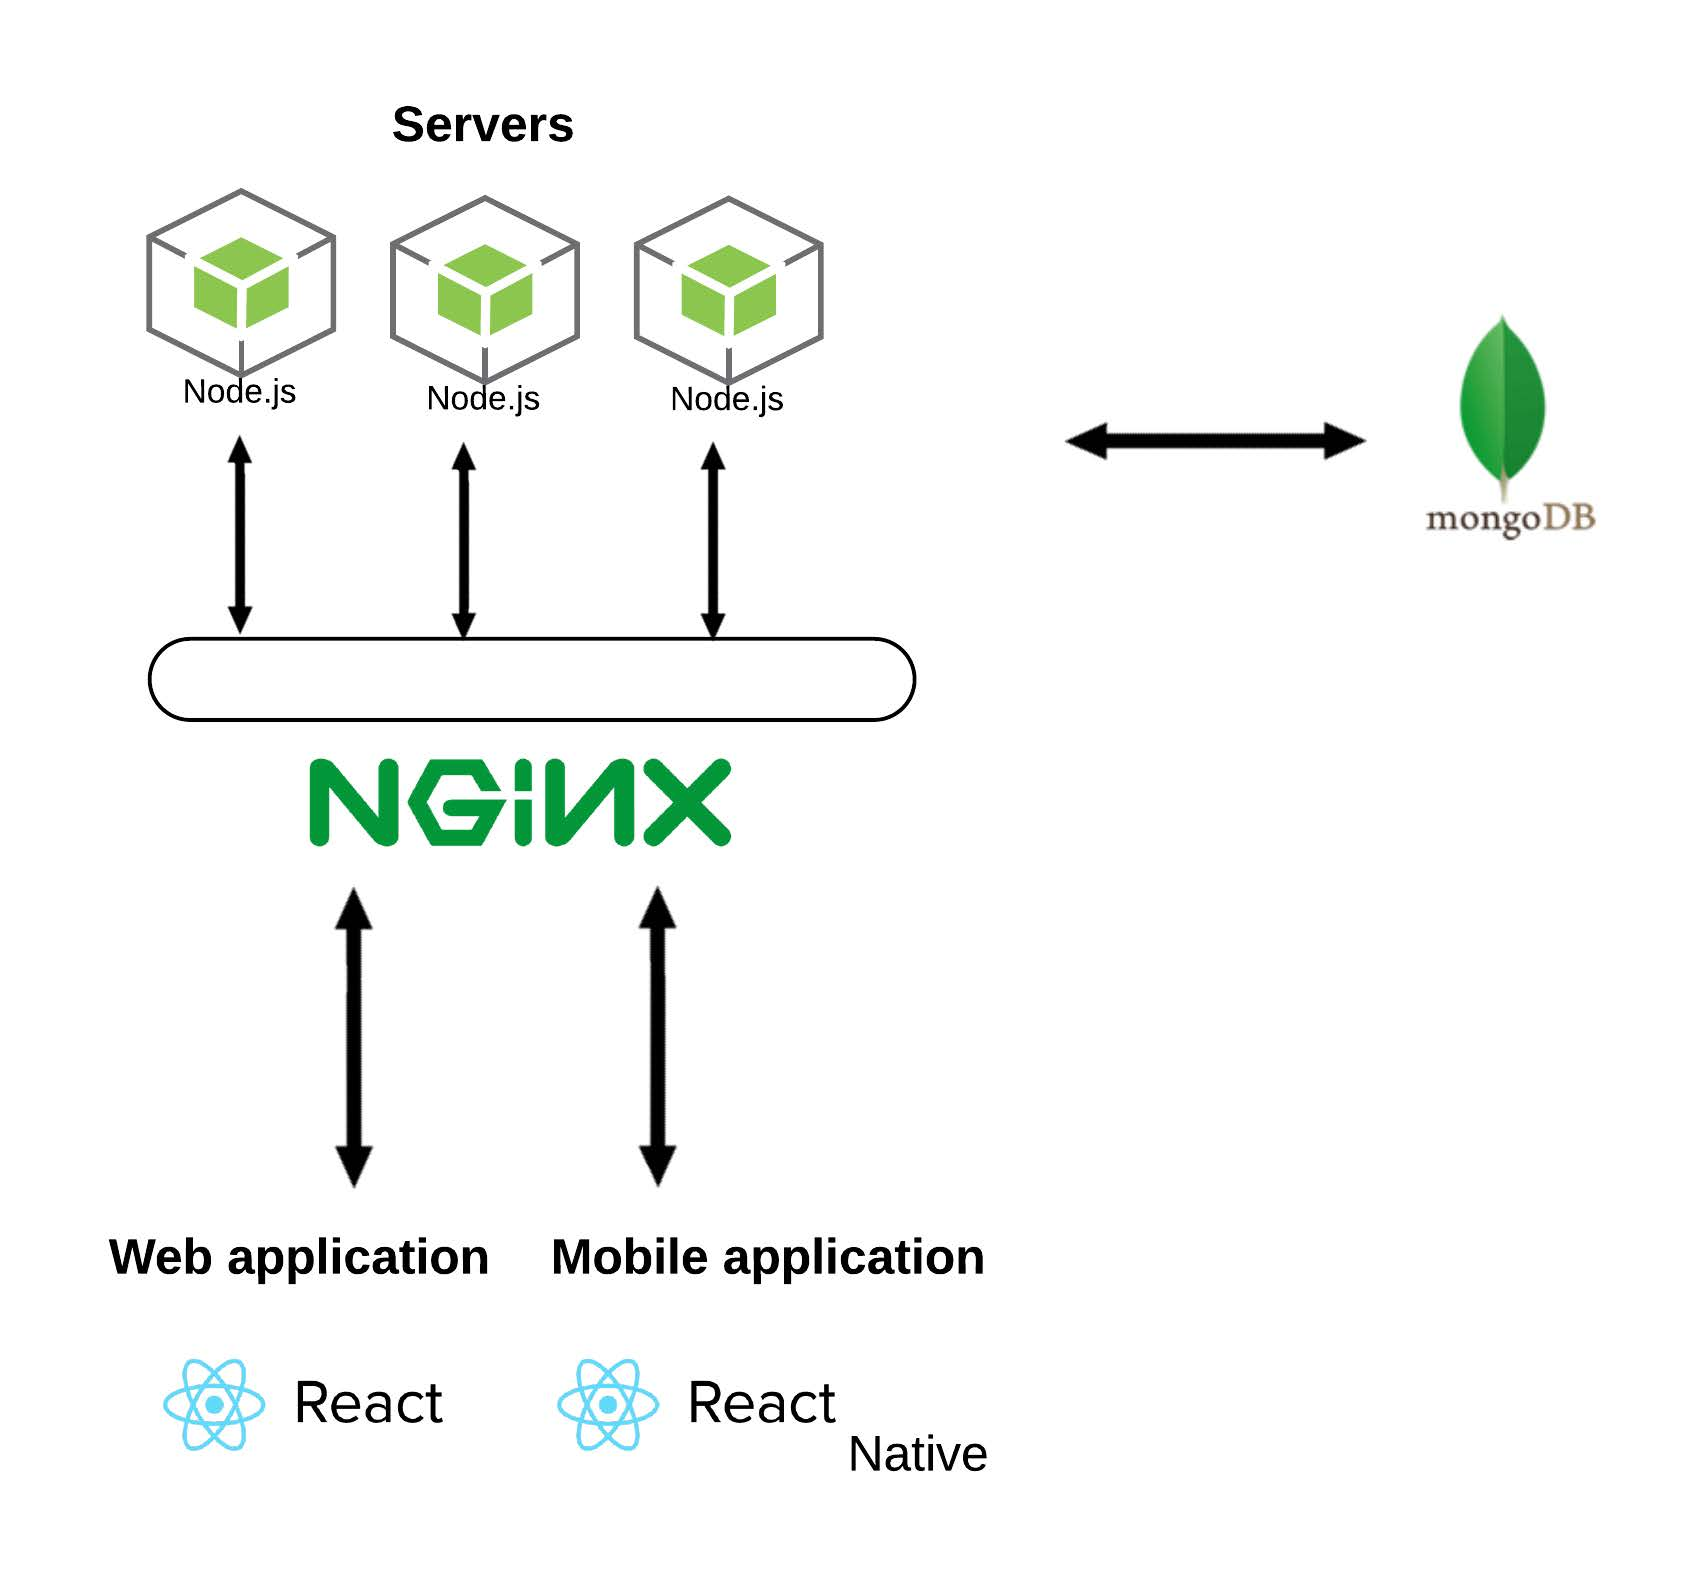
\includegraphics[scale=0.6]{figures/mongoDB-strucure.png}
    \caption{Φιλοσοφία πίσω από τη σχεδίαση της \tl{MongoDB}.}
    \label{mondodb}
\end{figure}

